\documentclass[a4paper,oneside]{Tptesi2}

\usepackage[italian]{babel}
\usepackage{listings}
\usepackage{amsmath,amssymb}
\usepackage{verbatim}
\usepackage{indentfirst}
\usepackage[utf8]{inputenc}
\usepackage{subfigure}
\usepackage{algorithmic}
\usepackage{framed}
\usepackage{rotating}
% ---------------- included packages by me
\usepackage{import}
\usepackage{bbm}
\usepackage{hyperref}
\usepackage{xcolor}
\usepackage{float}
\usepackage{enumitem}
\usepackage[rightcaption]{sidecap}
\usepackage{multicol}
\usepackage[sorting=none]{biblatex}
\addbibresource{biblio.bib}
\usepackage{csquotes}


\newcommand{\mr}{\emph{motore di ricerca}}
\newcommand{\Mr}{\emph{Motore di ricerca}}
\newcommand{\ws}{Web~service }


% Use a small font for the verbatim environment
\makeatletter  % makes '@' an ordinary character
\renewcommand{\verbatim@font}{%
  \ttfamily\footnotesize\catcode`\<=\active\catcode`\>=\active%
}
\makeatother   % makes '@' a special symbol again
%
% Simboli Matematici -------------------------------------------------------------
%\newcommand{\h}{\mathcal{H}_\infty} % scorciatoia per sequenza usata spesso
% Definizioni & Teoremi ----------------------------------------------------------
\newtheorem{teorema}{Teorema}[chapter]
\newtheorem{corollario}[teorema]{Corollario}
\newtheorem{lemma}[teorema]{Lemma}
%\theoremstyle{definition}
\newtheorem{definizione}{Definizione}[chapter]
\newtheorem{proposizione}[definizione]{Proposizione}
% Formattazione Figure -----------------------------------------------------------
\setcounter{topnumber}{3}
\setcounter{totalnumber}{3}
\def\topfraction{1}
\def\textfraction{0}
% Fuzz ---------------------------------------------------------------------------
%\hfuzz10cm %Non scassare linee che escono dal bordo

% ------------------------ listing package configuration
\definecolor{codegreen}{rgb}{0,0.6,0}
\definecolor{codegray}{rgb}{0.3,0.3,0.3}
\definecolor{codepurple}{rgb}{0.58,0,0.82}
\definecolor{backcolour}{rgb}{0.97,0.97,0.97}
% colors defined by me
\definecolor{code_blue}{rgb}{0.0, 0.4, 1}
\definecolor{code_green}{rgb}{0, 0.6, 0}
\definecolor{light_orange}{rgb}{1, 0.46, 0.1}
\definecolor{dark_orange}{rgb}{1, 0.20, 0.0}

\lstdefinestyle{pyStyle} {
  backgroundcolor=\color{backcolour},   
  commentstyle=\color{code_green},
  keywordstyle=\color{code_blue},
  numberstyle=\sffamily\tiny\color{codegray},
  stringstyle=\color{light_orange},
  basicstyle=\ttfamily\scriptsize,
  breakatwhitespace=false,   
  breaklines=true,                 
  captionpos=b
  keepspaces=true,                 
  numbers=left,                    
  numbersep=5pt,                  
  showspaces=false,                
  showstringspaces=false,
  showtabs=false,                  
  tabsize=1
}
\lstset{style=pyStyle}

% --------------------------------------- MATH OPERATOR CREATED BY MYSSELF
\DeclareMathOperator*{\argmax}{arg\,max}


% ===========================================================================================
% Frontespizio -------------------------------------------------------------------
       \title{Metodi di esplorazione finalizzati alla copertura di utenti mediante agenti autonomi}
       \author{Leonardo Guglielmi}
       \titolocorso{Ingegneria Informatica}
       \chair{Prof. Giorgio Battistelli}
       \numberofmembers{1} %numero dei relatori
       \degreeyear{2024/25}
       \numerocorrelatori{1} %numero dei correlatori
       \correlatori{Nicola Forti} % i correlatori separati da \\

%
% ---- Inclusioni (vedi piu` sotto per il comando "include" --------------
%\includeonly {introduzione,chapter1, chapter2}
%\includeonly {chapter1, chapter2, chapter3, chapter4, chapter5, chapter6}
%\includeonly{chapter6}
%
\hypersetup{%
%  pdfpagemode=FullScreen,%
  plainpages=false,%
  breaklinks,%
  pdftitle={},%
  pdfauthor={Leonardo Guglielmi},%
  pdfsubject={},%
  pdfkeywords={},%
  colorlinks=true,
  citecolor={blue},
  linkcolor={black},
  urlcolor={cyan}
}

\begin{document}

\frontmatter

%\hyphenation{}

\pagestyle{headings} % rende attive le impostazioni sulla testata!

\maketitle % crea il frontespizio (ricordati di copiare "stemma.eps" nella tua directory)


\pagenumbering{roman}
\section*{Abstract} \label{sec:asbtract}
\textit{
I sistemi multiagente, quali le reti UAV, sono un paradigma tecnologico molto diffuso che con il passare del tempo ha visto la sua adozione in diversi contesti applicativi.
Tra questi, si annovera quello della copertura di utenti mediante sistemi di telecomunicazione, specialmente in quei casi in cui la posizione e il numero di tali utenti sono ignoti.
Inserendosi in tale scenario, la seguente tesi si prefigge l'obiettivo di sviluppare un algoritmo di esplorazione dell'area di interesse finalizzato alla ricerca di utenti disposti a terra.
}
\section*{Introduzione} \label{sec:intro}

Le reti UAV sono dei sistemi che, grazie alla loro scalabilità, flessibilità e adattabilità, hanno trovato un grande impiego in numerosi ambiti, anche molto eterogenei tra loro, come le comunicazioni nelle fasi di soccorso \cite{GuanYue2024CUTD}; il monitoraggio delle coltivazioni \cite{farming}; il monitoraggio ambientale \cite{forest}; la sorveglianza \cite{JainRachna2021TaSS}; l'erogazione di servizi di comunicazione \cite{8675384}; l'esplorazione di pianeti \cite{planetaryExpl}; e molti altri.
In particolare essi possono formare una rete wireless aerea, con la possibilità di scambiarsi reciprocamente informazioni riguardanti l'ambiente circostante, la presenza di eventuali ostacoli, o la posizione di utenti a cui deve essere garantita la copertura di segnale: perciò, oltre alle comunicazioni UAV-to-UAV generalmente questo tipo di rete ha anche la capacità di comunicare con dispositivi localizzati a terra.
\newline
\newline
Partendo dal modello di copertura esaminato in \cite{tesiInnocenti}, e supponendo che il numero di utenti totali non sia noto, e che anzi potrebbe variare nel tempo, questa tesi si pone l'obiettivo di sviluppare un algoritmo di esplorazione collaborativo per reti UAV avente il compito di guidare i droni nell'esplorazione dell'area alla ricerca di nuovi utenti, e che al contempo riesca a garantire la copertura di segnale di quelli già connessi alla rete.

In letteratura esistono varie metriche su cui basarsi per costruire un algoritmo atto all'esplorazione di una regione.
Questo comporta che al variare della metrica cambi il comportamento medio che gli agenti esibiscono; per esempio alcuni algoritmi potrebbero avere come obiettivo la massimizzazione dell'estensione geografica coperta nel tempo (Mean Square Distance, MSD), favorendo la decisione da parte degli agenti di spostamenti lunghi, mentre altri algoritmi potrebbero concentrarsi sul disincentivare l'esplorazione ripetuta delle stesse aree (rilascio di feromoni virtuali, \cite{SchroederAdam2017Escb}).
La diversità di questi approcci comporta una serie di vantaggi e svantaggi nel loro utilizzo, che possono andare dal consumo energetico per gli spostamenti, alla reciproca interferenza tra il segnale degli agenti, alla flessibilità verso variazioni dell'ambiente.

In questo progetto si è deciso di sviluppare un algoritmo di esplorazione basandosi sulla probabilità che, nei punti dell'area di interesse non coperti dal sistema in un certo istante, vi possa essere un utente. Il sistema quindi, equipaggiato con tale algoritmo, si focalizzerà sul cercare di ridurre la probabilità media, sia aumentando la propria estensione totale, riducendo quindi le zone non coperte, sia visitando regioni con associata un'alta probabilità.



\section*{Struttura della tesi} \label{sec:struttura_tesi}

Il contenuto di questa tesi è strutturato nel seguente modo: all'interno del \textbf{capitolo 1} vengono introdotti alcuni concetti fondamentali, legati agli argomenti inerenti al contesto della tesi, quali una breve definizione di sistema multiagente e dei tipi di problema che vengono affrontati. Il \textbf{capitolo 2} si concentra sul presentare il modello matematico usato per formalizzare il problema e il sistema; successivamente nel \textbf{capitolo 3} si mostra l'implementazione dell'algoritmo di controllo e le strategie risolutive adottate.
Il \textbf{capitolo 4} riporta lo svolgimento degli esperimenti e l'analisi dei risultati da essi ottenuti.
Infine, nel \textbf{capitolo 5} vengono tratte le conclusioni sull'esperimento, soffermandosi anche su possibili futuri sviluppi della ricerca sul tema.
\tableofcontents % inserisce indice generale
\cleardoublepage

%\addcontentsline{toc}{chapter}{Elenco delle figure}
%\addcontentsline{toc}{chapter}{Elenco delle tabelle}
%\listoftables    % inserisce indice tabelle
%\addcontentsline{toc}{chapter}{Elenco degli algoritmi}
%\listofalgorithms

%
%--------------- Inizio del testo vero e proprio
%

\pagenumbering{arabic}

\mainmatter
\chapter{Copertura ed esplorazione multiagente} \label{ch:cov_expl_multiagent}
In questo capitolo viene data una spiegazione introduttiva dei sistemi presi in analisi e dei problemi che vengono affrontati.
\section{Caratteristiche dei sistemi multiagente} \label{sec:sistemi_multiagente}

I sistemi multiagente sono una classe di sistemi composti da un insieme entità autonome, dette agenti, capaci di interagire tra loro e con l'ambiente circostante.
La definizione di agente, come riporta \cite{WooldridgeMichaelJ.1966-2002Aitm}, non è unica e concordata universalmente, ma in generale può essere definito come \textit{un'unità situata in un ambiente, capace di eseguire delle azioni autonome, con la finalità di raggiungere un obiettivo prefissato}.

Un esempio naturale, a cui sono ispirati anche alcuni algoritmi di esplorazione, è rappresentato dalle colonie di formiche: in tali sistemi, migliaia di individui (agenti) agiscono in modo indipendente l'uno dagli altri, collaborando per la ricerca di cibo.
Ciascuna formica prende delle decisioni finalizzate al bene della colonia, basandosi sulla propria visione dell'ambiente che la circonda, e sulle informazioni trasmesse dai suoi simili tramite segnali chimici, come i feromoni.
\begin{figure}[h]
    \centering
    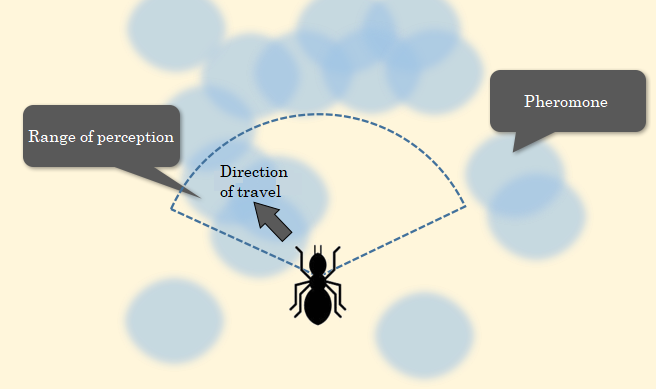
\includegraphics[width=0.6\textwidth]{img/ch1/esempio_formiche_tesi.png}
    \caption{Schema di comportamento di una formica.}
    \label{fig:schema_formica}
\end{figure}

A partire da questo esempio di sistema biologico, è possibile evidenziare alcuni elementi chiave dei sistemi multiagente:
\begin{itemize}

\item \textbf{Obiettivo}:
ogni agente ha un obiettivo e agisce in modo da raggiungerlo.

\item \textbf{Autonomia/Indipendenza}:
ogni agente compie delle scelte e delle azioni in modo autonomo rispetto agli altri agenti del sistema.

\item \textbf{Collaborazione}:
gli agenti possono collaborare tra loro per il raggiungimento di fini comuni nel caso che essi lo ritengano più utile al raggiungimento dell'obiettivo (non tutti i sistemi risultano collaborativi, si immagini per esempio, una partita di poker in cui ogni agente è un giocatore \cite{RussellStuartJ2022Ai:a}).

\item \textbf{Interazione con l'ambiente}:
ogni agente è in grado di interagire con l'ambiente circostante, sia per compiere azioni, sia per raccogliere informazioni propedeutiche alla scelta delle azioni da eseguire.

\item \textbf{Comunicazione}:
gli agenti possono avere dei sistemi per comunicare tra loro, con finalità di coordinazione o di scambio di informazioni.

\end{itemize}

Un'altra caratteristica fondamentale è quella dell' \textbf{ambiente} di essere \textbf{statico o dinamico}: nel primo caso si intende un ambiente che non varia nel tempo, anche a seguito delle azioni degli agenti, mentre per ambiente dinamico si intende un ambiente variabile nel tempo, e che dunque richiede un'analisi continua da parte degli agenti che lo abitano.

L'elenco esposto non è assolutamente esaustivo di tutte le proprietà che permettono la classificazione dei sistemi multiagente e del loro ambiente \cite{RussellStuartJ2022Ai:a}, dato il loro elevato numero si è deciso di evidenziare solo quelle più rilevanti per il caso d'analisi esaminato.

Analogamente all'esempio riportato precedentemente, il sistema multiagente utilizzato in questa tesi è un sistema collaborativo, con obiettivo globale e condiviso tra gli agenti, inserito all'interno di un ambiente parzialmente osservabile e dinamico, che varia sia in modo autonomo, sia a causa dell'azione degli agenti stessi.
 % 1.1
\section{Introduzione alle reti UAV} \label{sec:reti_uav}

% TODO ricontrolla chiarezza e fluidità di tutto il testo
I veicoli aerei senza pilota UAV (Unmanned Aerial Vehicle) sono dei mezzi volanti controllati da remoto, o in alcuni casi, completamente autonomi (Figura \ref{fig:esempi_uav}).
\begin{figure}[t]
    \centering
    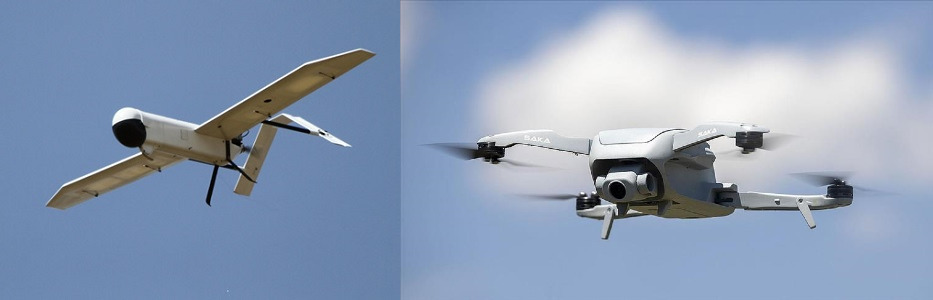
\includegraphics[width=0.8\textwidth]{img/ch1/esempi_uav.jpg}
    \caption{Esempi di dispositivi UAV}
    \label{fig:esempi_uav}
\end{figure}

Le reti UAV \cite{JavaidShumaila2023CaCi} sono dei sistemi multiagente composti da un insieme di \textbf{droni}, eventualmente anche da stazioni a terra (\textbf{Base Stations}, BS), capaci di comunicare tra di loro, che vengono usati come \textbf{nodi di una rete wireless} e svolgono la funzione di \textbf{ripetitori di segnale}; questo sistema è in grado di configurarsi in modo tale da fornire una connessione agli utenti dislocati a terra (Figura \ref{fig:esempio_rete_uav}).

L'adozione di questo paradigma per fornire accesso alla rete presenta diversi vantaggi, ad esempio:
\begin{itemize}

\item regolando l'altitudine dei droni è possibile aggirare agevolmente ostacoli presenti a terra, permettendo di stabilire collegamenti in linea d'area (Line of Sight, LoS)

\item la limitata necessità di strutture fisse a terra permette il dispiegamento dell'infrastruttura di rete in modo rapido, rendendola particolarmente adatta a situazioni di emergenza

\item data l'elevata mobilità dei nodi è possibile riconfigurare facilmente la rete a fronte di variazioni delle necessità da parte degli utenti, ottenendo un'alta flessibilità

\item data la struttura della rete si ha un'alta scalabilità del sistema

\end{itemize}

Un altro aspetto rilevante di questo paradigma è quello che, essendo presente una connessione tra gli agenti, è possibile l'interscambio di informazioni riguardanti l'area circostante di ciascun drone, riuscendo quindi a dare ad ogni singolo agente una visione più completa dell'area attualmente esplorata.

\begin{figure}[t]
    \centering
    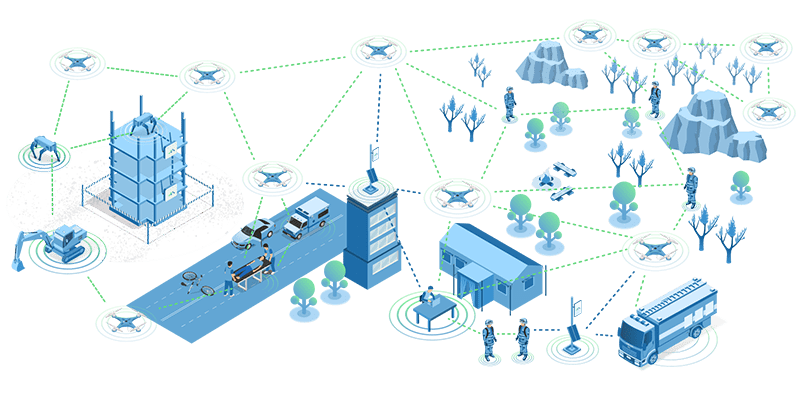
\includegraphics[width=1\textwidth]{img/ch1/uav_network_example.png}
    \caption{Esempio schematico di una rete UAV}
    \label{fig:esempio_rete_uav}
\end{figure}

Nelle reti di telecomunicazioni esistono diversi paradigmi per gestire la comunicazione tra i nodi della rete; uno degli aspetti caratterizzanti di questi paradigmi è la topologia adottata, ovvero la disposizione spaziale dei nodi e dei collegamenti fra di essi.
Per quanto riguarda le reti wireless UAV si possono adottare due tipi di topologie:
\begin{itemize}

\item \textbf{topologia centralizzata}:
ogni nodo deve avere un collegamento diretto con un elemento centrale della rete per essere connesso, ad esempio le BS. Questa tipologia pone in modo evidente un grosso limite all'esplorazione dell'area di interesse, in quanto gli agenti non potranno allontanarsi dai nodi centrali, limitando le zone esplorabili.

\item \textbf{topologia decentralizzata}:
non si identifica un nodo avente maggiore rilevanza, e affinché un nodo sia connesso non importa che abbia un collegamento diretto con un nodo master, ma è sufficiente che vi sia un collegamento indiretto. Questo approccio permette di disporsi in maniera più ampia nella regione da esplorare e di adottare una configurazione maggiormente mutabile nel tempo.
\end{itemize}
\begin{figure}
    \centering
    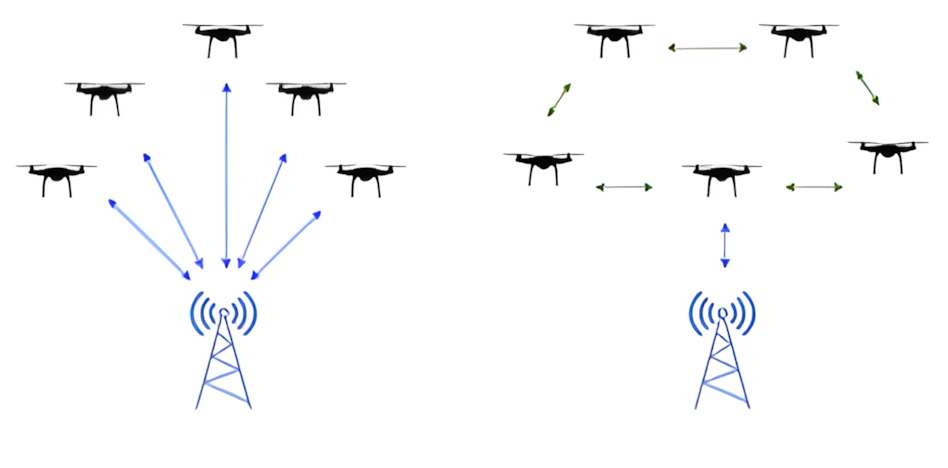
\includegraphics[width=0.8\textwidth]{img/ch1/uav_network_topology.png}
    \caption[Esempi di topologie di rete]{Confronto tra le due topologie di rete: a sinistra vengono mostrati schematicamente dei collegamenti tipici di un network UAV con topologia centralizzata; a destra, lo stesso sistema ma con topologia decentralizzata}
    \label{fig:uav_topology_example}
\end{figure}

Al fine di instaurare una connessione tra agenti può sembrare ragionevole utilizzare la stessa rete utilizzata per la comunicazione con gli utenti. 
Tale approccio tuttavia rischia di limitare l'efficienza complessiva, in quanto la tecnologia utilizzata nelle connessioni tra utenti ed agenti potrebbe non supportare comunicazioni a lunga distanza, riducendo di conseguenza la distribuzione geografica del sistema.
Una strada alternativa per gestire la comunicazione tra UAV può essere quella di utilizzare una rete apposita, detta rete di \textbf{backhaul} \cite{GuanYue2024CUTD}\cite{AlzenadMohamed2016FVBF}; questo comporta una divisione della rete complessiva in due sottoreti, in un certo grado indipendenti tra di loro.
Il vantaggio di utilizzare questa divisione è quello che la rete di backhaul può sfruttare tecnologie di telecomunicazioni a più ampio raggio, come ad esempio la Free Optical Space (FOS) \cite{8938182} o le comunicazioni satellitari \cite{HosseiniNozhan2020UCaC} (Figura \ref{fig:backhaul_example}), in modo che la comunicazione tra agenti non risulti un fattore limitante per la performance del sistema.
\begin{figure}[t]    
    \centering
    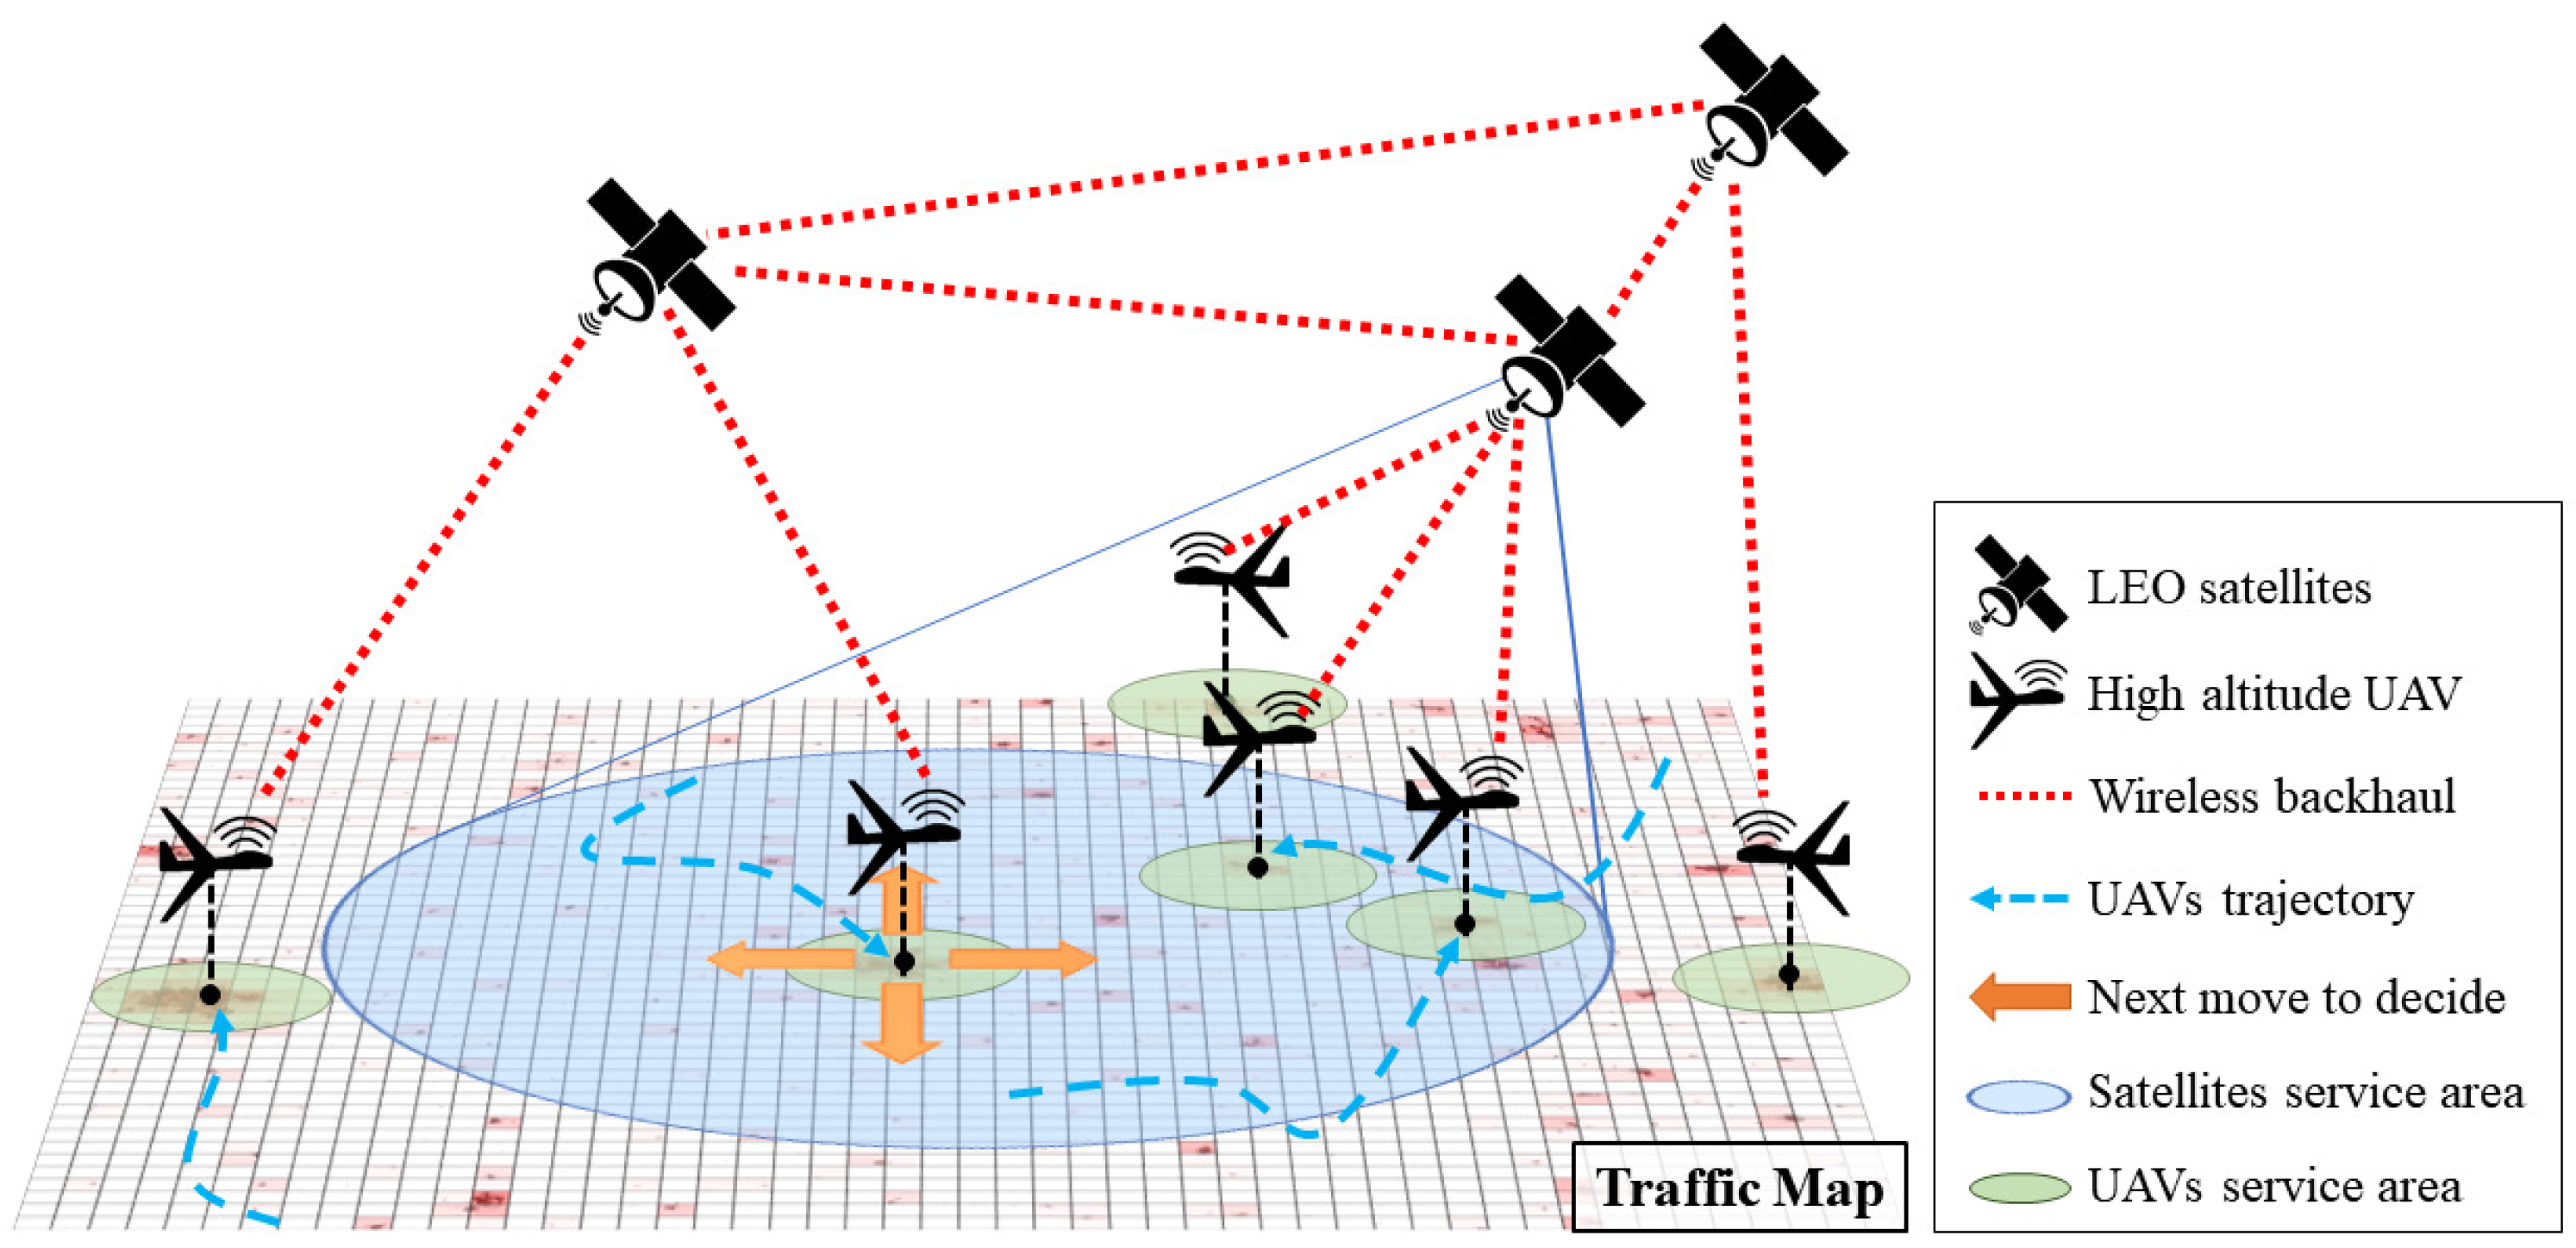
\includegraphics[width=1\textwidth]{img/ch1/satellite_backhaul_network_example.png}
    \caption[Comunicazioni UAV-to-UAV con backhaul satellitare]{Rappresentazione schematica delle comunicazioni UAV-UAV mediante una rete backhaul satellitare.}
    \label{fig:backhaul_example}
\end{figure} % 1.2
\section{Formulazione dei problemi} \label{sec:descr_problemi}

Nelle seguenti sezioni viene data una breve descrizione dei due principali problemi che verranno affrontati in questa tesi.
\subsection{Problema della copertura} \label{subsec:prob_copertura}

Si consideri un insieme di utenti, posizionati a terra, di cui non si conosce il numero complessivo né la posizione, a cui si deve fornire connessione tramite la rete di droni.
Il problema di copertura si pone l'obiettivo di trovare una disposizione delle fonti di segnale (droni ed eventuali BS) tale che il segnale ricevuto da ciascun utente noto soddisfi una serie di requisiti.

Il controllo della copertura può ricadere sotto due categorie: statico e dinamico. 
Nel primo, lo scopo è quello di trovare il  posizionamento ottimale degli agenti per garantire la copertura degli utenti, mentre il secondo usufruisce della mobilità delle fonti di segnale, cercando di connettere dei soggetti che possono muoversi nel tempo.
In questa tesi, l'algoritmo di copertura statico \cite{tesiInnocenti} utilizzato nel lavoro precedente è stato riadattato per renderlo compatibile con lo scenario in cui il numero totale di utenti non è noto.
\subsection{Problema dell'esplorazione} \label{subsec:prob_esplorazione}
Si consideri una regione in cui sono presenti alcuni elementi, ma di cui non si conoscono alcune informazioni; per esempio le posizioni degli utenti e il loro numero in un determinato istante di tempo.
Ci si pone quindi il problema di come, utilizzando le stesse fonti di segnale utilizzate per il problema di copertura, esplorare le porzioni di regione che in un determinato istante non sono coperte dal segnale della rete.

Come per la copertura, in ambito scientifico si vanno ad individuare due categorie di algoritmi per l'esplorazione di un'area: algoritmi statici, in cui si determina a priori il percorso che un agente deve percorrere affinché ogni zona della regione venga esplorata almeno una volta, pensati per contesti in cui l'ambiente non varia o le cui variazioni sono sufficientemente lente, e algoritmi dinamici, in cui invece l'esplorazione di una zona potrebbe ripetersi più volte nel tempo, al seguito della variazione di alcune condizioni (Figura \ref{fig:path_static_dynamic_environment}).

\begin{figure}[ht]
    \centering
    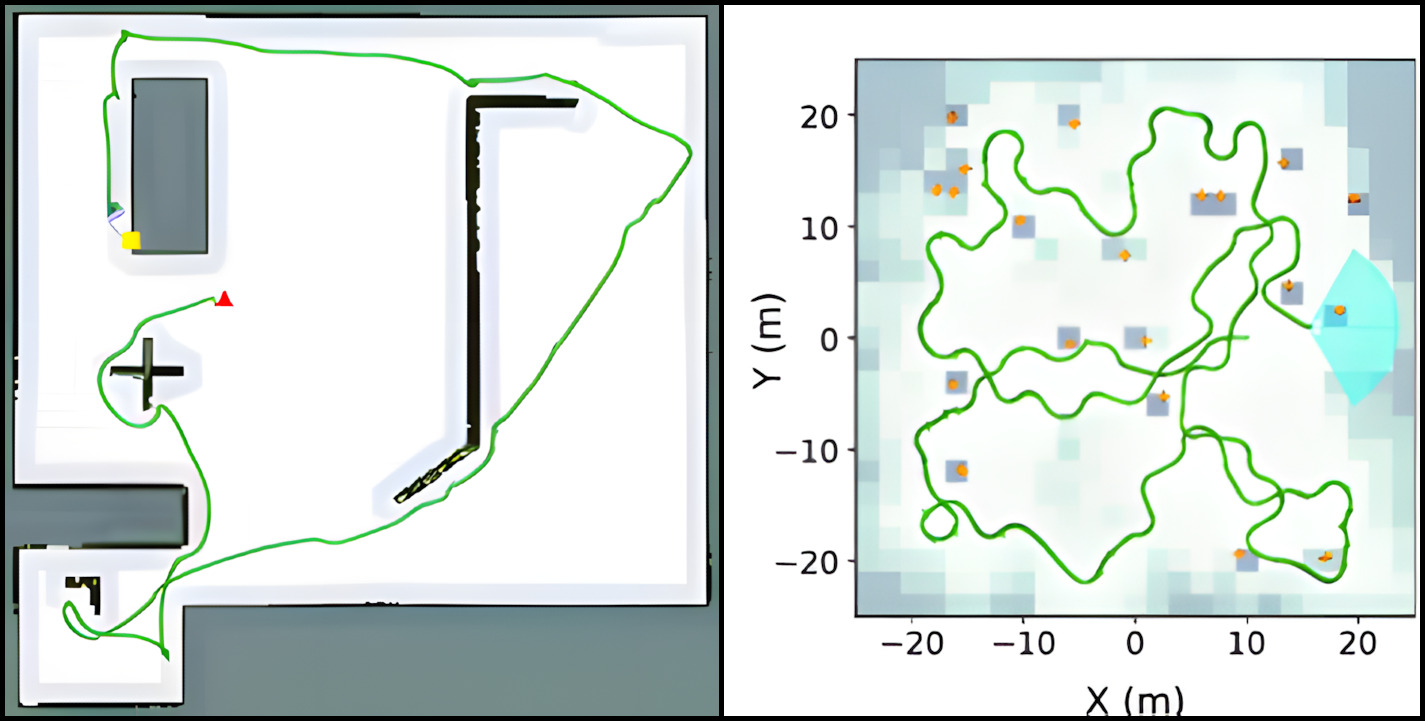
\includegraphics[width=0.9\textwidth]{img/ch1/path_dynamic_static_environment.jpg}
    \caption[Esempi di traiettorie in ambiente statico e dinamico]{Esempi di traiettorie in un processo di esplorazione: a sinistra,ù in ambiente statico; a destra in ambiente dinamico. Si osserva come l'ambiente dinamico provoca una traiettoria molto più caotica.}
    \label{fig:path_static_dynamic_environment}
\end{figure}
\pagebreak
In questa tesi si affronterà un problema in cui l'ambiente da esplorare verrà considerato dinamico, e quindi verrà adottato un algoritmo di esplorazione da eseguire ripetutamente nel tempo.
Si suppone infatti che all'interno della regione di interesse le posizioni degli utenti non siano note, e che il numero degli stessi possa variare: un nuovo utente quindi, posizionato in una zona già visitata ma non attualmente coperta, potrebbe richiedere la connessione alla rete, oppure un utente già presente e coperto potrebbe disconnettersi dalla rete.
 % 1.3
\chapter{Modello matematico} \label{ch:modello} % 2
In questo capitolo verranno formulati i modelli matematici del sistema, della copertura e dell'esplorazione. Inoltre, verrà presentato lo schema dell'algoritmo di controllo utilizzato negli esperimenti che seguiranno.
\section{Modello del sistema} \label{sec:modello_sistema}
Si considerino $M$ \textbf{utenti} a cui deve essere fornita connessione alla rete, distribuiti a terra all'interno di un'area bidimensionale $A$, con posizioni $u_j \in \mathbbm{R}^2 ,\ j \in \{1, ...M \}$.
Sono presenti $N$ \textbf{agenti} mobili UAV ed eventualmente $B$ \textbf{Base Stations}, aventi l'obiettivo di formare una rete mobile UAV e di fornire segnale agli utenti, mentre esplorano quelle porzioni di area che non sono coperte.
Si indicano con $x_i \in \mathbbm{R}^3 ,\ i \in \{1, ...N \}$ le posizioni degli agenti mobili, e con $b_k \in \mathbbm{R}^2 ,\ k \in \{1, ...B\}$ le posizioni delle BS.
Per limitare la problematica della connessione tra agenti, si ipotizza l'impiego di una rete di backhaul che permetta di considerare il grafo di connessione tra agenti sempre connesso.
D'ora in poi, per semplificare la trattazione, si userà il termine \textit{sensore} per indicare sia gli agenti mobili che le BS, in quanto entrambi hanno la capacità di fornire copertura ed esplorare.

Vengono quindi fatte le seguenti ipotesi sul sistema:
\begin{enumerate}

\item
il numero di agenti mobili è strettamente minore del numero di utenti, così come il numero di BS, se presenti, è minore di quello degli agenti: $B<N<M$

% ============================================================================================
% OLD GRAPH SENSOR NETWORK
% ============================================================================================
%\item 
%ciascun agente ha una capacità di comunicazione limitata, modellata mediante una sfera di raggio $R$ centrata nella posizione dell'agente; si ha che, affinché due sensori $i$ e $j$ possano comunicare direttamente, deve intercorrere una distanza $d(i,j)<R$

%\item
%la rete che si forma tra i sensori è modellata tramite un grafo indiretto $G=(V,E(t))$, dove $V$ rappresenta l'insieme dei nodi (agenti mobili e BS) mentre $E(t)$ rappresenta i collegamenti indiretti attivi tra i sensori; deriva dunque che, al tempo $t$, $(i,j)\in E(t)\iff d(i,j)<R$.

%\item
%la rete di sensori comunica mediante una topologia decentralizzata; ciò implica che sia sufficiente che il grafo sia connesso in ciascun istante $t$ 

\item
al fine di evitare collisioni, gli agenti sono disposti ad altitudini diverse, da cui si ha che, per un sensore $i$ e un utente $j$, $d_{i,j}(t)=\sqrt{||x_i - u_j ||^2 + h_i^2}$

\item
tra sensori e utenti vengono considerati i collegamenti LoS

\end{enumerate} % 2.1
\section{Modello di copertura} \label{sec:modello_copertura}

Nei problemi di copertura ci sono vari requisiti ed indicatori su cui basare la funzione obiettivo; in questa tesi si considera come obiettivo del problema di copertura la massimizzazione del \textbf{Region Coverage Ratio} (RCR), ossia il rapporto tra il numero di utenti coperti $M_C$ e il numero totale di utenti $M_D$ di cui si conosce l'esistenza:
\begin{equation}
    RCR = \frac{Mc}{M_D}
\end{equation}

Per quantificare il livello di copertura di un utente da parte di un sensore si è deciso di usare il \textbf{Signal to Interference plus Noise Ratio}, definito tra un sensore $i$ e un utente $j$ come:
\begin{equation}
    \gamma_{i,j}(t)=\frac{\psi_i(t)g_{i,j}(t)}{\mu_{i,j}(t)+\beta\nu_0}
\end{equation}
I termini che compaiono nell'equazione sono:
\begin{itemize}
    \item
        $\psi_i(t)$ è la potenza di trasmissione del sensore $i$

    \item
        $g_{i,j}(t) = \frac{\rho_0}{d_{i,j}(t)}$ rappresenta il guadagno di canale al tempo $t$ tra il sensore $i$ e l'utente $j$, con $\rho_0$ guadagno del collegamento, $d_{i,j}(t)$ la distanza tra i due elementi 

    \item
        $\mu_{i,j}(t)=\sum_{k\in N\setminus\{i\}} \psi_k(t)g_{k,j}(t)$ è la potenza di interferenza relativa al collegamento $(i, j)$, dovuta alle interferenze tra sensori

    \item
        $\beta$ è la larghezza di banda del canale, $\nu_0$ è la Power Spectral Density of Noise (PSDN)
    
\end{itemize}

Usando questo modello per il SINR, si definisce l'RCR come:
\begin{equation}
    C(t) = \frac{\sum_{j=1}^{M_D}c_j(t)}{M_D} = \frac{\sum_{j=1}^{M_D}\mathbbm{1}(\gamma_j(t)-\tau)}{M_D}
\end{equation}
con $\tau$ rappresenta il valore di soglia oltre al quale un utente è considerato coperto, $\gamma_j(t)=\max\limits_{i=1...N}\{\gamma_{i,j}(t)\}$ e $\mathbbm{1}(x)$ è la funzione indicatrice. % 2.2
\section{Modello di esplorazione} \label{sec:modello_esplorazione}
% espandi questa sezione
% MY STUFF --------------------------------------------------------------------------------
In questa tesi si pone come obiettivo del problema di esplorazione quello di minimizzare la probabilità media che un utente possa trovarsi in una regione non coperta dal segnale di un sensore.
Per questo motivo, si divide l'area di interesse in $K$ celle uguali, e a ciascuna cella $k$, se non coperta, si associa la probabilità $P_k(t)$ che al suo interno vi sia un utente.
A tal proposito si definiscono:
\begin{itemize}
    \item $\mathbbm{P}_D$ come la probabilità che un utente già connesso alla rete si disconnetta

    \item $\mathbbm{P}_B$ come la probabilità che un nuovo utente voglia connettersi alla rete     
\end{itemize}
si definisce quindi la probabilità associata alla cella $k$ nell'istante $t$ come:
\begin{equation}
    \label{eq:prob_cella}
    P_k(t) = \begin{cases}
        \bar{P_k}(t-1)\ \mathbbm{P}_B + P_k(t-1)\ (1-\mathbbm{P}_D) \text{ se } k \text{ non coperta} \\
        0 \text{ se } k \text{ coperta}
    \end{cases}
\end{equation}
dove $\bar{P_k}$ è la proprietà complementare di $P_k$, ovvero $\bar{P_k} = 1-P_k$.
Variando i valori di $\mathbbm{P}_B$, $\mathbbm{P}_D$ è possibile modificare la variabilità dell'ambiente, adattandolo allo scenario reale qualora si abbiano alcune informazioni a priori su di esso.
Inoltre, al fine di avere un \textit{feedback} sull'effettiva copertura degli utenti nella fase di esplorazione, si va a porre ad 1 la probabilità di una cella qualora essa contenga un utente che, a seguito di una variazione della disposizione degli agenti, passi dallo stato coperto allo stato non coperto.

Come criterio di valutazione della copertura di una cella si è deciso di adottare lo stesso usato nel problema di copertura degli utenti; si va quindi a considerare il \textbf{SINR} calcolato nel \textbf{centro} della cella, riassumendo la probabilità in quella regione con quella del suo centro, e considerandola coperta quando $\gamma_k(t)>\tau'$, dove $\gamma_k(t)=\max\limits_{i=1...N}\{\gamma_{i,k}(t)\}$ e $\tau'$ è la soglia minima richiesta.

Definendo in tal modo la probabilità associata a ciascuna cella, si definisce il \textbf{livello di esplorazione globale} dell'area $A$ come:
\begin{equation}
    \label{eq:global_funct}
    \Pi(t) = 1 - \frac{\sum_k P_k(t)}{K}
\end{equation}
in tal modo, minimizzando la probabilità media, si va ad aumentare il livello di esplorazione, trasformando quindi il problema di minimo in un problema di massimo e rendendolo compatibile con il problema di copertura.
 % 2.3
\section{Algoritmo di controllo} \label{sec:algoritmo_controllo}
L'algoritmo di controllo ha il compito di indirizzare ciascun agente verso quelle zone che massimizzano la funzione obiettivo $R(t)$, considerando anche le posizioni degli altri agenti.
In questo progetto la funzione obiettivo si compone di due contributi: l'obiettivo di copertura, che mira a massimizzare l'RCR degli utenti noti, e l'obiettivo di esplorazione, che cerca di massimizzare il livello di esplorazione (o in altri termini, di diminuire la probabilità media).
Per combinare i due obiettivi, i valori di copertura ed esplorazione vengono sommati, applicando a quest'ultimo un coefficiente $\rho$, il quale indica la rilevanza dell'esplorazione all'interno dell'obiettivo globale:
\begin{equation}
    \label{eq:objective_function}
    R(t) = C(t) + \rho\ \Pi(t)
\end{equation}

Schematicamente, l'algoritmo di controllo si articola nei seguenti passaggi:
\begin{enumerate}
    \item 
    per ogni agente, campiona \texttt{NUM\_SAMPLES} punti nello spazio, secondo una certa distribuzione di probabilità, successivamente ciascuno di essi viene selezionato o scartato secondo una certa regola.
    Formalmente, date le posizioni $x_1...x_N\in \mathbbm{R}^3$ degli agenti nel tempo $t$, a ognuno di essi viene associato un insieme di punti $S_i\subset A$.

    \item
    per ogni agente $i$, si individua tra i punti $p_i\in S_i$ quello che, se assunto come nuova posizione dell'agente, massimizzerebbe $R(t)$, ovvero $p^*_i=\argmax\limits_{p_i\in S_i} R(t)$, valutando quindi per ogni punto campionato $C(t)$ e $\Pi(t)$.

    \item
    All'istante successivo $t+1$ si muove l'agente $i$ verso il suo punto obiettivo $p_i^*$, aggiornando la sua posizione secondo la formula:
    \begin{equation}
        x_i(t+1) = \begin{cases}
            x_i(t)+\varepsilon\delta_i\ \ \ \ \text{ se } \varepsilon||\delta_i||<\Delta \\
            x_i(t)+\Delta \cfrac{\delta_i}{||\delta_i||}\ \ \ \ \text{ altrimenti}
        \end{cases}
    \end{equation}
    dove $\delta_i=p_i^*-x_i$ è la distanza tra il punto obiettivo e la posizione attuale dell'agente; $\varepsilon\in(0,1)$ è la percentuale di spostamento che l'agente compie verso l'obiettivo; $\Delta\in 
    % qui milgiora
    \mathbbm{R}$ è la massima distanza che un agente può percorrere ad ogni iterazione. Limitando la massima distanza di spostamento si evita di perturbare eccessivamente la configurazione, favorendo la coordinazione del sistema \cite{PangBao2021Eorw}. 

    \item 
    l'algoritmo ripete i punti precedenti per \texttt{NUM\_OF\_ITERATIONS} iterazioni.
\end{enumerate}

La natura iterativa di questo algoritmo permette agli agenti di coordinarsi tra di loro: in ciascuna iterazione ogni agente rivaluta la propria direzione al seguito dello spostamento degli altri agenti, evitando di esplorare zone più facilmente raggiungibili da altri e migliorando la resa del sistema in termini di esplorazione e copertura utente.
Affinché l'algoritmo possa funzionare correttamente si rende necessario l'utilizzo di alcune strutture dati, che verranno aggiornate a ciascuna iterazione: più precisamente, è necessaria una lista contenente gli utenti noti al tempo $t$, e una matrice che divida l'area in celle e associ a ciascuna di queste la relativa probabilità.

Osservando il bilanciamento dei due obiettivi all'interno di $R(t)$ durante la fase di valutazione di $p_i^*$ per ciascun agente si nota come il livello di copertura non possa mai essere maggiore di 1, ed è minore solo nei casi in cui un agente, spostandosi, non riesca più a coprire uno o più utenti.
Applicando il coefficiente $\rho$ al valore di esplorazione si riducono le possibilità che ciò accada, evitando che si perdano completamente informazioni su alcuni utenti e favorendo quindi la copertura di quelli noti.
Tuttavia, tale perdita è concessa nel caso in cui il guadagno in termini di esplorazione sia molto alto. % 2.4
\chapter{Implementazione} \label{ch:implementazione} % 3

In questo capitolo viene discussa l'implementazione dei modelli presentati nel capitolo \ref{ch:modello}, evidenziando le diverse strategie adottate per affrontare alcune problematiche.
In particolar modo, verrà data rilevanza alle tecniche e alle strutture dati impiegate nel calcolo dell'esplorazione, riportando le varianti utilizzate durante il processo di sperimentazione del modello, quali i vari metodi di valutazione del guadagno di esplorazione di un punto campionato da un agente (Sezione \ref{sec:valutazione_esplorazione}).

Il codice del sistema e delle simulazioni, così come la cronologia delle modifiche, è disponibile su GitHub nel seguente repository: 

\href{https://github.com/leonardo-guglielmi/Multiagent-exploration-system.git}{\textsf{https://github.com/leonardo-guglielmi/Multiagent-exploration-system.git}}

Il linguaggio di programmazione utilizzato è 
%\href{https://www.python.org/about/}{\textbf{Python}}, 
\textbf{Python}, 
che grazie alla sua semplicità e alla vasta gamma di librerie disponibili si rende particolarmente adatto alle fasi prototipali di un progetto.

\section{Schema del progetto} \label{sec:schema_classi}

In Figura \ref{fig:uml_scheme} si riporta il diagramma UML delle classi del progetto (per la sua realizzazione è stato utilizzato il tool online 
%\href{https://app.diagrams.net/}{\textbf{draw.io}}
\textbf{draw.io}).

\begin{figure}[p]
    \centering
    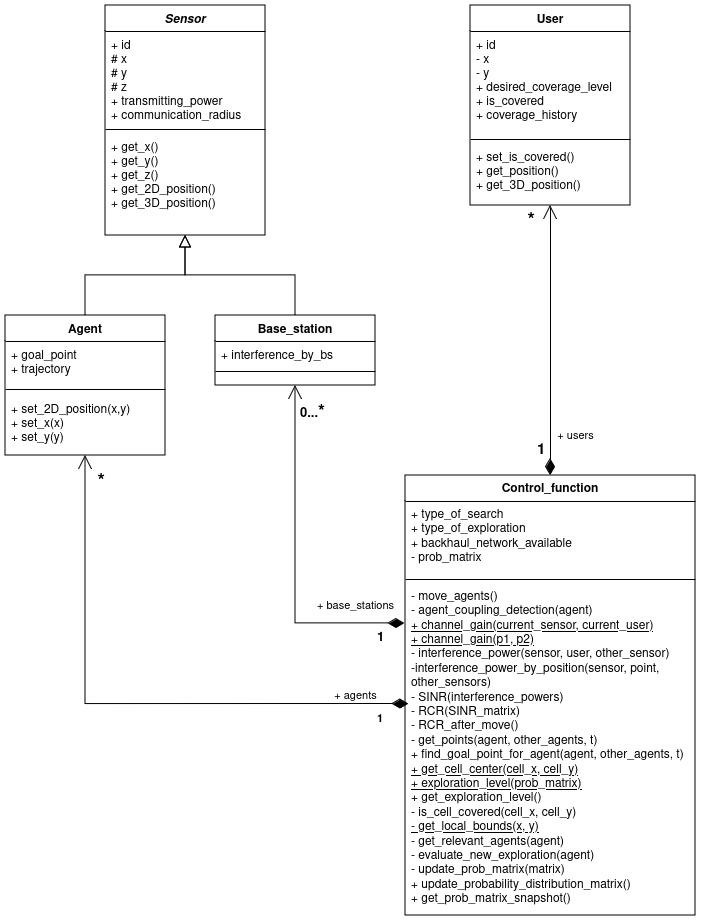
\includegraphics[width=1\textwidth]{img/ch3/UML_thesis.png}
    \caption[Schema UML]{Schema UML della classi usate nella simulazione}
    \label{fig:uml_scheme}
\end{figure}

\subsection{Classi \texttt{Sensor, Agent e Base\_stations}} \label{subsec:sensors}
La classe \texttt{Sensor} rappresenta un sensore, astraendo le differenze tra agente e BS.
Contiene le caratteristiche comuni ai due elementi del sistema, ovvero la posizione tridimensionale \texttt{(x,y,z)}; la potenza di trasmissione \texttt{trasmitting\_power}; il raggio di esplorazione \texttt{exploration\_radius}, implementati come attributi della classe.
La classe \texttt{Agent} estende \texttt{Sensor}, aggiungendovi gli attributi propri degli agenti, ovvero \texttt{trajectory}, una lista cronologica delle posizioni occupate dall'agente, e \texttt{goal\_point}, il punto obiettivo che l'agente vuole raggiungere in un certo istante di tempo.
La classe \texttt{Base\_station} estende anch'essa \texttt{Sensor}, ed aggiunge semplicemente un attributo booleano \texttt{interference\_by\_bs}: se impostato a \texttt{True}, indica che il segnale di quella BS interferisce con quello degli \texttt{Agent}. Questo flag è stato aggiunto poiché, in molti casi reali, le frequenze sui cui operano i due sensori sono diverse e non interferiscono tra di loro. % 3.1.1
\subsection{Classe \texttt{User}} \label{subsec:user}

La classe \texttt{User} rappresenta un utente a terra a cui deve essere fornita copertura.
Gli attributi rilevanti sono la posizione \texttt{(x,y)}; il livello di SINR \texttt{desired\_coverage\_level} tale che l'utente sia considerato coperto; il booleano \texttt{is\_covered}, che indica se in un certo istante di tempo tale utente è coperto o meno; una lista \texttt{coverage\_history} che contiene la cronologia dello stato di copertura dell'utente nel tempo. % 3.1.2
\subsection{Classe \texttt{Control\_function}} \label{subsec:control_function}
Questa classe contiene i metodi utilizzati dalla funzione di controllo.
Al suo interno sono presenti i riferimenti a tutti gli attori del sistema: troviamo infatti una lista di \texttt{Agent}, una di \texttt{Base\_station} e una di \texttt{User}.
Inoltre, contiene tutta una serie di attributi usati durante i processi decisionali, come il criterio per la scelta tra i punti campionati, oppure la matrice di probabilità utilizzata per l'esplorazione, descritta meglio in  \ref{subsec:mappa_prob}.

\subsubsection{Metodo  \texttt{move\_agents()}}
Questa funzione, mostrata nello Snippet \ref{snip:move_agents}, esegue lo spostamento degli agenti come descritto in \ref{sec:algoritmo_controllo}.
Inoltre, nel caso in cui venga riconosciuta una situazione di accoppiamento tra agenti, viene applicata una deviazione; tale processo è descritto approfonditamente in \ref{sec:controllo_accoppiamento_agenti}.

\lstinputlisting[
    language=Python 
    , label= {snip:move_agents}
    , caption = {Funzione per lo spostamento degli agenti.}
    , frame=tb
    , belowcaptionskip=3mm
    , float = h
    ]
{code/move_agent_snip.py}

\subsubsection{Metodo \texttt{get\_points()}}
Dato un agente, questa funzione campiona un insieme di punti e ne restituisce un sottoinsieme secondo una certa regola.
Più precisamente, vengono campionati \texttt{NUM\_OF\_SAMPLES} punti secondo una \textbf{distribuzione normale}, centrata nell'attuale posizione dell'agente specificato.
Le strategie di selezione dei punti adottate sono le seguenti:
\begin{enumerate}

\item
Ricerca \textbf{systematic}: vengono considerati tutti i punti campionati. 
Questa strategia ha il problema che, occasionalmente, restituisce dei punti lontani dall'agente, e se tra questi vi fosse il punto ottimo, porterebbe l'agente a muoversi verso zone che, probabilmente, verrebbero esplorate prima da altri agenti, rendendo lo spostamento vano.

\item
Ricerca \textbf{local}: tra i punti campionati, vengono selezionati solo quelli che sono più vicini all'agente specificato rispetto ad altri sensori (Snippet \ref{snip:local_search}). Questa strategia predilige quindi un controllo locale dell'area, impedendo che un sensore vada a esplorare una zona che è più facilmente esplorabile da un altro.

\lstinputlisting[
    language=Python 
    , label= {snip:local_search}
    , caption = {Tecnica di selezione \textit{local}.}
    , frame=tb
    , belowcaptionskip=3mm
    , float = t
    ]
{code/local_search_snip.py}

\item
Ricerca \textbf{penalty}: come nella strategia \textit{local}, questa tecnica favorisce quei punti prossimi all'agente. A differenza della precedente non va ad escludere quelli più vicini ad altri, bensì va ad applicare una penalità ai livelli di $C(t)$ e $\Pi(t)$ calcolati in tali punti.

\pagebreak
\item
Ricerca \textbf{annealing forward}: riprendendo l'idea dell'algoritmo di ricerca locale \textit{simulated annealing}, si va ad aggiungere alla strategia \textit{local} una probabilità aggiuntiva, decrescente con il tempo, che il punto venga selezionato anche se è più vicino ad altri agenti. %(Snippet \ref{snip:annealing_search}).
Questa tecnica cerca di evitare lo stallo in punti di massimo locale.

\item
Ricerca \textbf{annealing reverse}: simile alla ricerca \textit{annealing forward}, in questa tecnica si va ad avere una probabilità crescente nel tempo. %(Snippet \ref{snip:annealing_search}).
In questo modo, con il passare del tempo, il valore atteso della lunghezza degli spostamenti aumenterà.
\end{enumerate}

%\lstinputlisting[
%    language=Python 
%    , label= {snip:annealing_search}
%    , caption = {Tecnica di selezione \textit{annealing forward} e \textit{annealing reverse}}
%    , frame=tb
%    , belowcaptionskip=3mm
%    , float = t
%    ]
%{code/annealing_search_snip.py}

\subsubsection{\texttt{find\_goal\_point\_for\_agent()}}
Dato un agente, questo metodo esamina tutti i punti forniti da \texttt{get\_points()}, più la posizione attuale dell'agente, cercando tra di essi l'ottimo.
Per fare ciò la posizione del sensore viene temporaneamente modificata con quella del punto in esame e viene ricalcolata la funzione obiettivo nella nuova configurazione del sistema; nel caso in cui il valore ottenuto sia il migliore trovato tale punto viene salvato come nuovo $p_i^*$.
Poiché la funzione obiettivo, come esposto nel capitolo \ref{ch:modello}, si divide in due parti, per valutare $R(t)$ nel nuovo punto dovranno essere calcolati nuovamente l'RCR e il valore di esplorazione.

\subsubsection{\texttt{is\_cell\_covered()}}
Questo metodo, fornite le coordinate di una cella di esplorazione, ritorna lo stato di copertura di quest'ultima.
Come indicato in \ref{sec:modello_esplorazione}, per determinare lo stato si prende come punto di riferimento il centro della cella; questo implica un'approssimazione sulla reale probabilità che in quella zona vi sia un utente, approssimazione che cresce all'aumentare della dimensione delle celle.

\input{files/ch3/classi progetto/mappa_probabilità}
\input{files/ch3/classi progetto/funzione_esplorazione} % 3.1.3 % 3.1
\section{Esecuzione concorrente} \label{subsec:concur_agents}

In un contesto reale, ciascun agente eseguirebbe la funzione obiettivo sul proprio sistema di calcolo in modo indipendente dagli altri.
Si è dunque ritenuto opportuno implementare un meccanismo di parallelizzazione per il calcolo del \texttt{goal\_point} di ciascun agente, riducendo sensibilmente i tempi di esecuzione delle simulazioni.
Data la presenza nell'interprete Python del \textit{Global Interpreter Lock}, la scelta del modulo da impiegare è ricaduta su \texttt{multiprocessing}, un package Python che espone delle API per la creazione e gestione di processi paralleli.

 Per parallelizzare la simulazione, si crea un processo distinto per ciascun agente, il quale eseguirà il metodo \texttt{goal\_point\_agent()}.
 Una volta calcolato il punto ottimo, il processo lo inserisce in un dizionario condiviso, associandogli come chiave l'id del proprio agente.
Una volta terminati tutti i processi agente, nel processo principale viene estratto dal dizionario ciascun \texttt{goal\_point} e associato al relativo agente (Snippet \ref{snip:concurrent_simu}).
\lstinputlisting[
language=Python 
, label = {snip:concurrent_simu}
, caption = {Esecuzione parallela della ricerca del \texttt{goal\_point}.}
, float = t
, frame = tb
, belowcaptionskip = 3mm
]{code/concurrent_simu.py} % 3.2
\section{Valutazione dell'esplorazione} \label{sec:valutazione_esplorazione}
Come accennato in \ref{subsubsec:expl_funct}, andare a valutare per ogni punto campionato l'esplorazione \textbf{globale} risulta estremamente costoso, implicando dei tempi di simulazione estremamente lunghi.
Inoltre, l'uso di questo approccio è poco utile; infatti dopo il movimento degli agenti nelle zone lontane dal punto campionato in esame avrò verosimilmente uno stato di esplorazione diverso, rendendo la previsione fatta su quelle celle durante la valutazione del punto ottimo poco attendibile.
A fronte di queste problematiche, durante le fasi sperimentali sono stati progettati e implementati diversi metodi per valutare localmente il livello di esplorazione di un punto, in modo che tale operazione risulti computazionalmente valida.

% metto prima il metodo finale, e poi le caratteristiche di quellli vecchi le ricollego a queste?
\subsection{Metodi sperimentali per la valutazione dell'esplorazione} \label{subsec:experimental_expl_eval}
In questa sotto-sezione si riportano i vari metodi sviluppati durante le fasi di test, ma che sono stati rimpiazzati da una versione successiva più accurata, fino ad arrivare a quello utilizzato negli esperimenti, ed esposto in \ref{subsec:expl_eval_frontier_NCC}.

\subsubsection{Simple Exploration}
Questo metodo è stato utilizzato nelle fasi iniziali per verificare la variazione di probabilità delle celle in tempi di simulazione ragionevoli. 
Esso non tiene conto del SINR per valutare la copertura di un cella, ma controlla soltanto che il suo centro sia abbastanza vicino ad un sensore.
Per ovvi motivi, tale metodo è stato rapidamente sostituito dai successivi.

\subsubsection{Local Square Interference Exploration (LSIE)}
In questa variante, si va a valutare la copertura di una cella tramite il livello di SINR calcolato nel suo centro, rendendo il requisito di copertura della cella simile a quello della copertura utente.
La novità principale è quella di non considerare tutte le celle della matrice, ma soltanto quelle che rientrano all'interno di un'area quadrata centrata nella posizione dell'agente, di lato \texttt{2$\cdot$EXPLORATION\_RADIUS} (Figura \ref{fig:esempio_LSIE}).
\begin{SCfigure}[1][h]
    \centering
    \caption[Esempio dell'area valutata con il metodo LSIE]{Esempio dell'area considerata dal metodo LSIE; si osserva come le celle presenti negli angoli dell'area siano difficilmente raggiungibili dal segnale dell'agente.}
    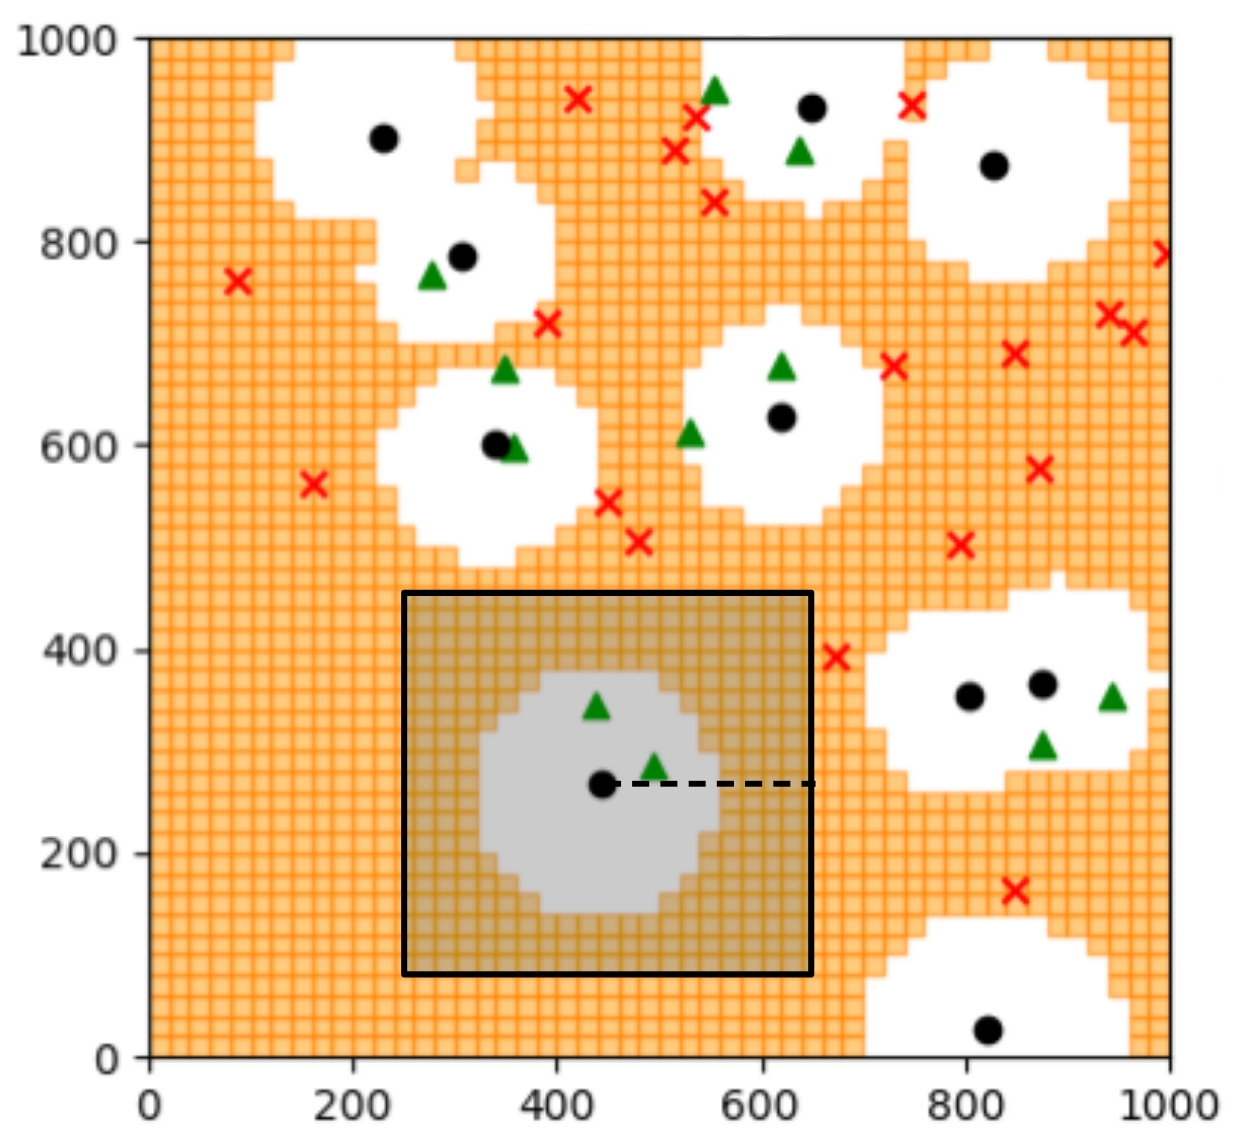
\includegraphics[width=0.5\textwidth]{img/ch3/esempio_LSIE.jpg}
    \label{fig:esempio_LSIE}
\end{SCfigure}

Inoltre si vanno a considerare soltanto le interferenze provenienti da sensori relativamente vicini all'agente, in quanto una eccessiva distanza rende il segnale d'interferenza trascurabile; questa considerazione permette di avere un minor numero di agenti nel calcolo del SINR, alleggerendo il costo computazionale.
Si osserva come la scelta del valore di \texttt{EXPLORATION\_RADIUS} sia critica, in quanto  un raggio maggiore implica una visione più approfondita dell'ambiente da parte dell'agente, comportando però una minore velocità del metodo.
\textbf{Sperimentalmente} si è osservato che ponendo \texttt{EXPLORATION\_RADIUS=200} si ha un'esplorazione completa dell'area intorno ad un punto, mantenendo un buon tempo di simulazione.
Il problema di questa variante è che, data la forma quadrata dell'area, si andranno a considerare anche le celle negli angoli, che molto probabilmente non saranno mai coperte dal segnale dell'agente (Figura \ref{fig:esempio_LSIE}).


\subsubsection{Local Circle Interference Exploration (LCIE)}
Rispetto al metodo precedente questa variante modifica la forma dell'area osservata, passando dall'utilizzo di un'area quadrata ad una circolare, rimuovendo quindi le celle che prima si trovavano negli angoli; questo porta ad un'ulteriore aumento di velocità del processo di valutazione, essendosi ridotto il numero di celle da osservare.
\begin{figure}[h]
    \centering
    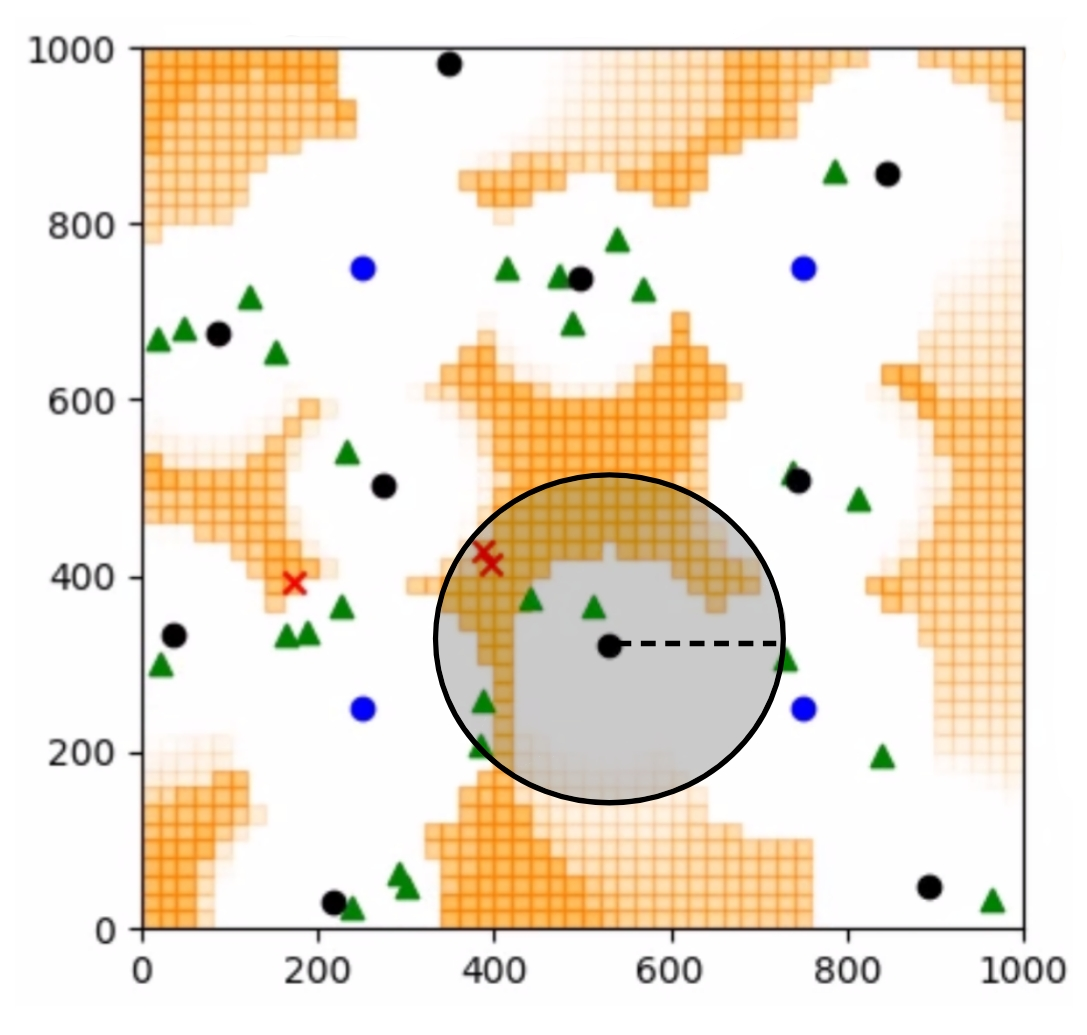
\includegraphics[width=0.5\textwidth]{img/ch3/esempio_LCIE.jpg}
    \caption[Esempio dell'area valutata con il metodo LCIE]{Esempio di area considerata dal metodo LCIE.}
    \label{fig:esempio_LCIE}
\end{figure}

\subsubsection{Local Square Interference Exploration, Neighbour Cell Control (LSIENCC)}
Implementata prima della \textit{Local Circle Interference Exploration}, questo metodo aggiunge una predizione sul livello di copertura di alcune celle quando sono soddisfatte alcune condizioni.
Tale predizione si basa sull'osservazione che, se il SINR calcolato in una cella è abbastanza alto, allora con molta probabilità anche quello delle celle adiacenti supererà la soglia richiesta.
Seguendo tale euristica, è possibile ridurre drasticamente i tempi di valutazione dell'esplorazione di quegli agenti isolati rispetto al resto della rete: infatti, la distanza da gli altri agenti fa sì che il livello di SINR rimanga abbastanza uniforme lungo l'area.
\subsection{Valutazione dell'esplorazione tramite frontiera con controllo delle celle adiacenti} \label{subsec:expl_eval_frontier_NCC}
Il metodo riportato in questa sotto-sezione è quello che verrà usato nelle simulazioni esposte nel Capitolo \ref{ch4:simulazioni}.
Esso è la combinazione delle varianti \textit{LCIE} e \textit{LSIENCC}, esposte nella sotto-sezione precedente; tale metodo include dunque i vantaggi di avere una regione da valutare il più ridotta possibile, senza però rinunciare alla precisione della stima, e di poter predire il livello di copertura di alcune celle, senza doverne calcolare esplicitamente il valore.

% da ricontrollare
I passaggi principali in cui l'algoritmo si articola sono i seguenti:
\begin{enumerate}[wide]


\item
Per prima cosa, il metodo seleziona quelle celle che rientrano nell'area da valutare, inserendo le informazioni rilevanti (posizione del centro e probabilità) in una struttura dati simile ad una matrice, ma con lunghezza delle righe variabile (Snippet \ref{snip:init_expl_eval}).
Inoltre, identifica gli agenti abbastanza vicini al punto campionato.
\lstinputlisting[
language=Python 
, label={snip:init_expl_eval}
, caption={Inizializzazione del metodo LCIENCC.}
, frame=tb
, float = ht
, belowcaptionskip=3mm
]{code/init_expl_eval_method.py}


\item
Successivamente, per ogni cella inclusa, calcola il SINR di ciascun agente precedentemente selezionato.
Dal calcolo del SINR vengono escluse quelle celle aventi $P_k=0$,  in quanto sono già coperte, e non apporterebbero nessun contributo all'esplorazione (Snippet \ref{snip:core_expl_eval}).
Se il livello di SINR di una cella supera una certa soglia \texttt{NEIGHBOUR\_SINR\_THRESHOLD}, la cella sovrastante e quella a destra (quella sotto e quella a sinistra sono state già esaminate) vengono inserite in \texttt{already\_checked\_cells}, ossia una lista che permette di escludere tali celle dalla valutazione del livello di SINR.
Prima di tale inserimento, viene fatta una serie di controlli per escludere quelle celle che eccedono l'aera di valutazione, e per evitare di etichettare come coperta una cella avente probabilità zero. 
\lstinputlisting[
language=Python 
, label={snip:core_expl_eval}
, caption={Calcolo della copertura nel metodo LCIENCC.}
, frame=tb
, float = p
, belowcaptionskip=3mm
]{code/core_expl_eval_method.py}


\item
Infine si calcola il livello di esplorazione, basandosi sulla matrice che associa a ciascuna cella il valore di SINR di ogni agente. (Snippet \ref{snip:final_expl_eval}).
\lstinputlisting[
language=Python 
, label={snip:final_expl_eval}
, caption={Valutazione dell'esplorazione nel metodo LCIENCC.}
, frame=tb
, float = h
, belowcaptionskip=3mm
]{code/final_expl_eval_method.py}


\end{enumerate} % 3.3
%\pagebreak
\section{Peso dell'esplorazione variabile} \label{sec:peso_esplorazione}
Il termine $\rho$, presente nell'Equazione \ref{eq:objective_function}, è un coefficiente che  indica l'importanza del processo di esplorazione all'interno dell'obiettivo globale.
Poiché la copertura degli utenti è l'obiettivo primario, inizialmente si è deciso di dare all'esplorazione una rilevanza minore, in modo che vengano favorite quelle azioni maggiormente orientate alla copertura; è stato dunque impostato un \textbf{peso constante} \texttt{EXPLORATION\_WEIGHT} (Snippet \ref{snip:expl_weight}), strettamente minore di 1.

\lstinputlisting[
language=Python 
, label={snip:expl_weight}
, caption = {varianti di peso dell'obiettivo di esplorazione}
, float = h
, frame=tb
, belowcaptionskip=3mm
]{code/expl_weight.py}

Successivamente è stato osservato come, nelle fasi iniziali, solitamente il valore di RCR fosse basso, risultando quindi sfavorevole incentivare la copertura di pochi utenti, rispetto alla ricerca di nuovi.
Per evitare tale comportamento, è stato implementato un \textbf{coefficiente di esplorazione decrescente} al crescere del numero di utenti coperti (Snippet \ref{snip:expl_weight}), ma indipendente dal loro totale, che permette di dare una rilevanza maggiore all'obiettivo di esplorazione nelle fasi iniziali, e ridurne il peso all'aumentare degli utenti coperti, applicando nuovamente un approccio più conservativo.
Inizialmente, come si vede in Figura \ref{fig:expl_weight_comparison}, quando la configurazione dei sensori ha un livello di RCR basso, l'importanza della funzione di esplorazione sarà relativamente elevata, per poi decrescere rapidamente; così facendo si ottiene un approccio flessibile alla configurazione attuale del sistema.

\begin{figure}
    \centering
    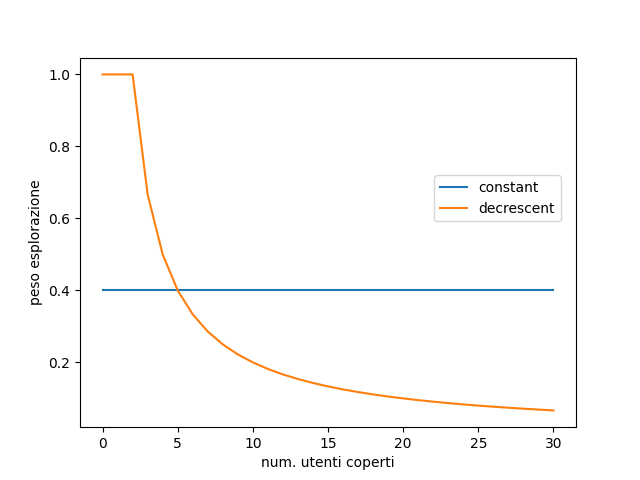
\includegraphics[width=0.8\textwidth]{img/ch3/expl_weight_comparison.png}
    \caption{Confronto tra i due tipi di peso al variare del numero di utenti coperti}
    \label{fig:expl_weight_comparison}
\end{figure}
\pagebreak
\section{Controllo per il disaccoppiamento di agenti} \label{sec:controllo_accoppiamento_agenti}

L'accoppiamento è un fenomeno causato dalla ridotta distanza tra due o più agenti, e provoca una minore capacità di copertura ed esplorazione da parte dei soggetti coinvolti.
Tale problematica si verifica quando agenti molto vicini identificano ripetutamente la stessa direzione di spostamento, causando un allineamento delle loro traiettorie; questo fa sì che il loro raggio di copertura si riduca a causa delle interferenze mutue.
Ciò ha come effetto quello di restringere l'orizzonte osservabile dagli agenti e conseguentemente un aumento della probabilità che gli agenti selezionino lo stesso punto ottimo.

\begin{figure}[t]
    \centering
    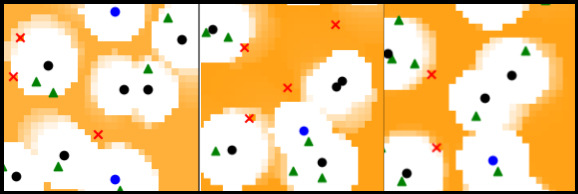
\includegraphics[width=0.8\textwidth]{img/ch3/agent_coupling_event.png}
    \caption[Esempio di accoppiamento tra agenti]{Un esempio di agenti accoppiati, rispettivamente negli istanti 15, 50 e 95. Si vede come, anche se la problematica sembra risolversi alla fine, essa ha drasticamente limitato il contributo degli agenti coinvolti.}
    \label{fig:agent_coupling_event}
\end{figure}

Per cercare di limitare la durata dell'accoppiamento è stato implementata una funzione in grado di riconoscere l'evento ed intervenire, cercando di orientare gli agenti coinvolti in direzioni opposte (Snippet \ref{snip:coupling_detection}).
\pagebreak
L'algoritmo implementato riconosce l'accoppiamento controllando ad ogni iterazione le posizioni pregresse degli agenti, confrontando le distanze mutue con un valore di soglia; nel caso questo venga raggiunto si crea una deviazione che cerca di allontanare gli agenti coinvolti.

\begin{SCfigure}[0.7][h]
    \centering
    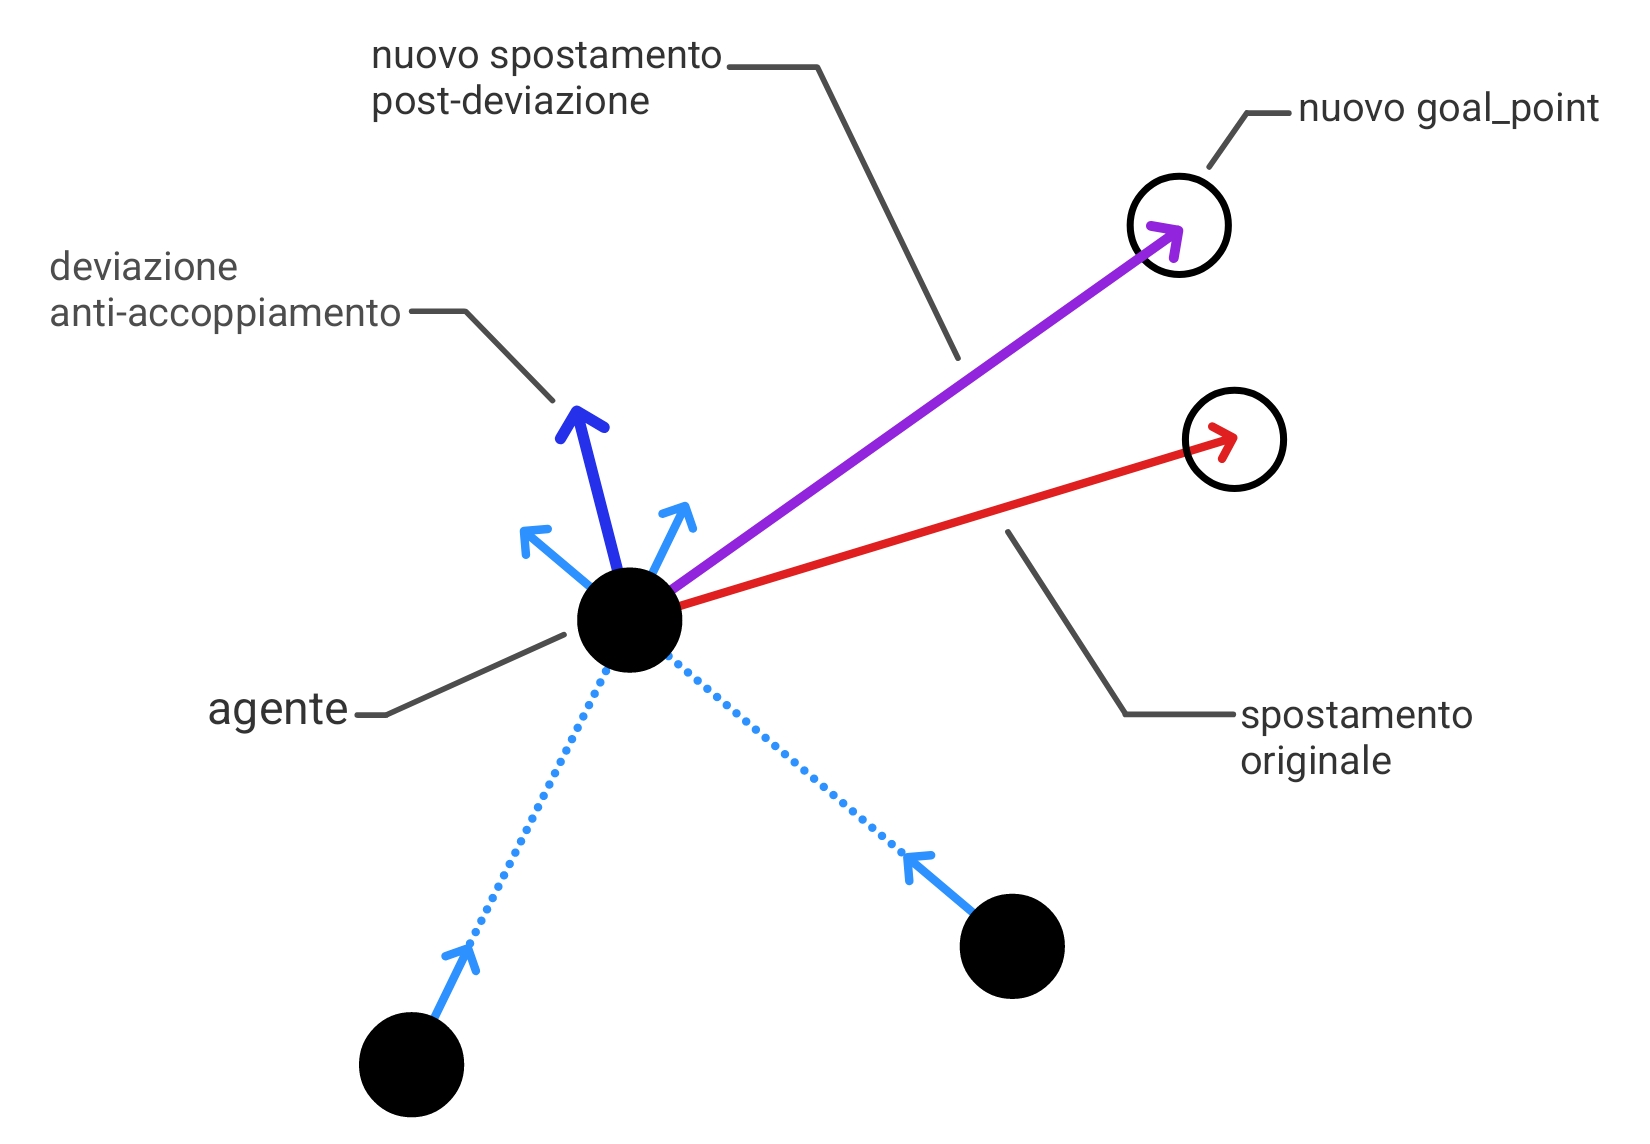
\includegraphics[width=0.6\textwidth]{img/ch3/schematic_anticoupling_system.jpg}
    \caption{Rappresentazione schematica del sistema anti-accoppiamento}
    \label{fig:schematic_decoupling_system}
\end{SCfigure}


Tale deviazione viene applicata sommandola alla direzione di spostamento del punto ottimo, come se fosse presente una forza repulsiva che agisce quando degli agenti sono vicini da troppo tempo (Figura \ref{fig:schematic_decoupling_system}).

\lstinputlisting[
    language=Python 
    , label= {snip:coupling_detection}
    , caption = {Funzione per il riconoscimento dell'accoppiamento.}
    , frame=tb
    , belowcaptionskip=3mm
    , float = p
    ]
{code/coupling_detection_system.py} % 3.4

\chapter{Simulazioni} \label{ch4:simulazioni}
Di seguito vengono descritti gli esperimenti svolti e le relative simulazioni, riportando e valutando i risultati.
\section{Valori dei parametri} \label{sec:param_vals}
Il valore dei parametri del sistema e del modello di copertura sono stati presi da \cite{valoriForti}, in modo da avere simulazioni il più vicino possibile a uno scenario reale.

\underline{Costanti del sistema}:
\begin{multicols}{2}
\begin{itemize}

\item \texttt{NUM\_OF\_SAMPLES =} 250

\item \texttt{NUM\_OF\_ITERATIONS =} 100

\item \texttt{AREA\_WIDTH =} 1000 m

\item \texttt{AREA\_LENGTH =} 1000 m

\item \texttt{MIN\_VERTICAL\_DISTANCE =} 0.15 m

\item \texttt{ALTITUDE =} 50 m, ovvero la minima altitudine dei droni

\item \texttt{MIN\_VERTICAL\_DISTANCE =} 0.15 m

\item \texttt{N =} 10, \texttt{B =} 4, \texttt{M =} 30

\end{itemize}
\end{multicols}

\underline{Parametri del modello di copertura}:
\begin{multicols}{2}
\begin{itemize}

\item \texttt{PSND =} 7.164$e^{-16}$ mW/Hz, che corrisponde a - 174 dBm/Hz ($\nu$)

\item \texttt{BANDWIDTH =} 2 MHz ($\beta$)

\item \texttt{PATH\_GAIN    =} $\frac{\lambda^2}{(4\pi)^2}$ = 0.0001, dove $\lambda=\frac{c}{f}$ è la lunghezza d'onda del segnale

\item \texttt{TRANSMITTING\_POWER =} 0.2 W ($\psi_i$) uguale per tutti i sensori

\item \texttt{DESIRED\_COVERAGE\_LEVEL =} 0.5 ($\tau$) uguale per tutti gli utenti

\end{itemize}
\end{multicols}

\underline{Costanti di movimento}:
\begin{multicols}{2}
\begin{itemize}

\item \texttt{EPSILON =} 0.1 ($\varepsilon$)

\item \texttt{MAX\_DISPLACEMENT =} 10 m ($\Delta$)

\end{itemize}
\end{multicols}

\underline{Parametri del modello di esplorazione}:
\begin{itemize}

\item \texttt{EXPLORATION\_CELL\_WIDTH =} 20 m

\item \texttt{EXPLORATION\_CELL\_HEIGTH =} 20 m

\item \texttt{EXPLORATION\_RADIUS =} 200 m

\item \texttt{EXPLORATION\_WEIGHT =} 0.4 ($\rho$)

\item \texttt{USER\_APPEARANCE\_PROBABILITY =} 0.015 ($\mathbb{P}_N$)

\item \texttt{USER\_DISCONNECTION\_PROBABILITY =} 0.008 ($\mathbb{P}_D$)

\item \texttt{INIT\_PROBABILITY =} 0.5, ovvero la probabilità iniziale di ciascuna cella

\item \texttt{NEIGHBOUR\_SINR\_THRESHOLD =} 0.85, ovvero il valore SINR di soglia oltre al quale considero come coperte anche le celle adiacenti

\item \texttt{DECOUPLING\_HISTORY\_DEPTH =} 5, ovvero il numero di posizioni della traiettoria che considero per la verifica dell'accoppiamento

\item \texttt{COUPLING\_DISTANCE =} 3$\cdot$\texttt{EXPLORATION\_CELL\_WIDTH}, ovvero la distanza minima al di sotto del quale considero due agenti accoppiati in un certo istante

\end{itemize} % 4.1
\section{Simulazioni e analisi dei risultati} \label{sec:res_analisys}
Le simulazioni sono state eseguite su una macchina Asus Vivobook S15 avente le seguenti caratteristiche: processore Intel Core i7-8565U 4 core 1.8 GHz; 8GB di RAM; SSD Kingstone da 256 GB.

Tutti i risultati degli esperimenti, come i grafici di andamento medio o le animazioni delle singole simulazioni, sono disponibili sul repository GitHub del progetto \href{https://github.com/leonardo-guglielmi/Multiagent-exploration-system.git}{\textsf{https://github.com/leonardo-guglielmi/Multiagent-exploration-system.git}}.

Negli esperimenti che seguono per ciascun tipo di scenario sono state effettuate 30 prove, ognuna con una configurazione delle posizioni iniziali degli agenti e degli utenti assegnata in modo casuale secondo una distribuzione uniforme lungo l'area di interesse.

\pagebreak
\subsection{Esperimento 1: verifica dell'efficacia dell'algoritmo di esplorazione}\label{subsec:exp1}
In questo esperimento si vuole verificare che l'algoritmo di esplorazione apporti effettivamente un miglioramento in termini di RCR totale rispetto al solo algoritmo per la copertura.
Per confermare ciò sono state effettuate delle simulazioni alternando l'esecuzione del metodo di esplorazione e la presenza delle BS, per un totale di 4 scenari diversi per ciascuna simulazione eseguita, utilizzando la tecnica di campionamento \textit{local}.


Nelle Tabelle  \ref{tab:exp1_cov_statistics}, \ref{tab:exp1_expl_statistics}  si mostrano alcuni indici statistici sui valori finali di RCR ed esplorazione raggiunti, mentre in Figura  \ref{fig:confronto_cov_exp1}, \ref{fig:confronto_expl_exp1}  vengono confrontati gli andamenti medi delle due grandezze durante le simulazioni.
Si osserva che, quando in uso, l'algoritmo di esplorazione effettivamente porta ad avere dei valori finali di copertura migliori. Si nota invece che quando esso non viene eseguito, una volta raggiunta una certa configurazione gli agenti smettono di muoversi, in quanto l'algoritmo di controllo non permette loro di abbandonare la copertura di alcuni utenti per la ricerca di altri, limitando quindi il numero massimo di utenti raggiungibili; a fronte di questo, si ipotizza dunque che se si fosse aumentato il numero di iterazioni di ciascuna simulazione, negli scenari con esplorazione si sarebbero potuti raggiungere valori di copertura migliori.
\begin{table}[t]
\begin{tabular}{|c|c|c|c|c|}
\hline
Simulazione & Massimo & Minimo & Media & Dev. standard \\
\hline
Esplorazione con BS & 0.97 & 0.73 & 0.87 & 0.0645 \\
No esplorazione con BS & 0.93 & 0.63 & 0.79 & 0.0756\\
Esplorazione senza BS & 0.87 & 0.63 & 0.75 & 0.0677 \\
No esplorazione senza BS & 0.8 & 0.5 & 0.64 & 0.0848 \\
\hline
\end{tabular}
\caption{\label{tab:exp1_cov_statistics}Primo esperimento, indici dei valori finali di copertura}
\end{table}

Inoltre, per fornire una migliore interpretazione dei dati, si fa presente che nelle simulazioni senza BS, nella maggior parte dei casi, il numero di agenti risulta troppo basso per avere una qualsiasi configurazione tale da permettere la copertura di tutti gli utenti.

\begin{figure}
    \centering
    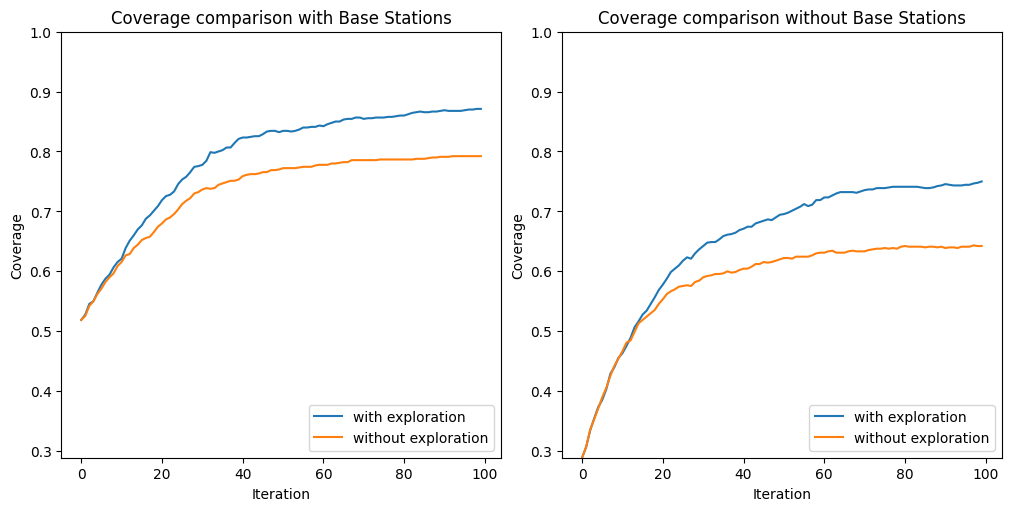
\includegraphics[width=1\textwidth]{img/ch4/experiment1/coverage_comparison.png}
    \caption[Grafici di copertura nel primo esperimento]{Confronto tra gli andamenti medi della copertura negli scenari di simulazione del primo esperimento.}
    \label{fig:confronto_cov_exp1}

    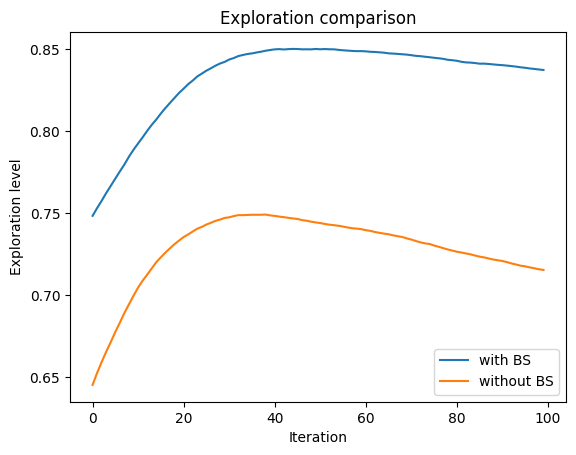
\includegraphics[width=0.5\textwidth]{img/ch4/experiment1/exploration_comparison.png}
    \caption[Grafici di esplorazione nel primo esperimento]{Confronto tra gli andamenti medi dell'esplorazione negli scenari di simulazione del primo esperimento.}
    \label{fig:confronto_expl_exp1}
\end{figure}

\begin{table}[t]
\centering
\begin{tabular}{|c|c|c|c|c|}
\hline
Simulazione & Massimo & Minimo & Media & Dev. standard \\
\hline
Con BS & 0.87 & 0.81 & 0.83 & 0.0129 \\
Senza BS & 0.76 & 0.67 & 0.71 & 0.0198 \\
\hline
\end{tabular}
\caption{\label{tab:exp1_expl_statistics}Primo esperimento, indici dei valori finali di esplorazione.}
\end{table}

\begin{figure}[p]
    \centering
    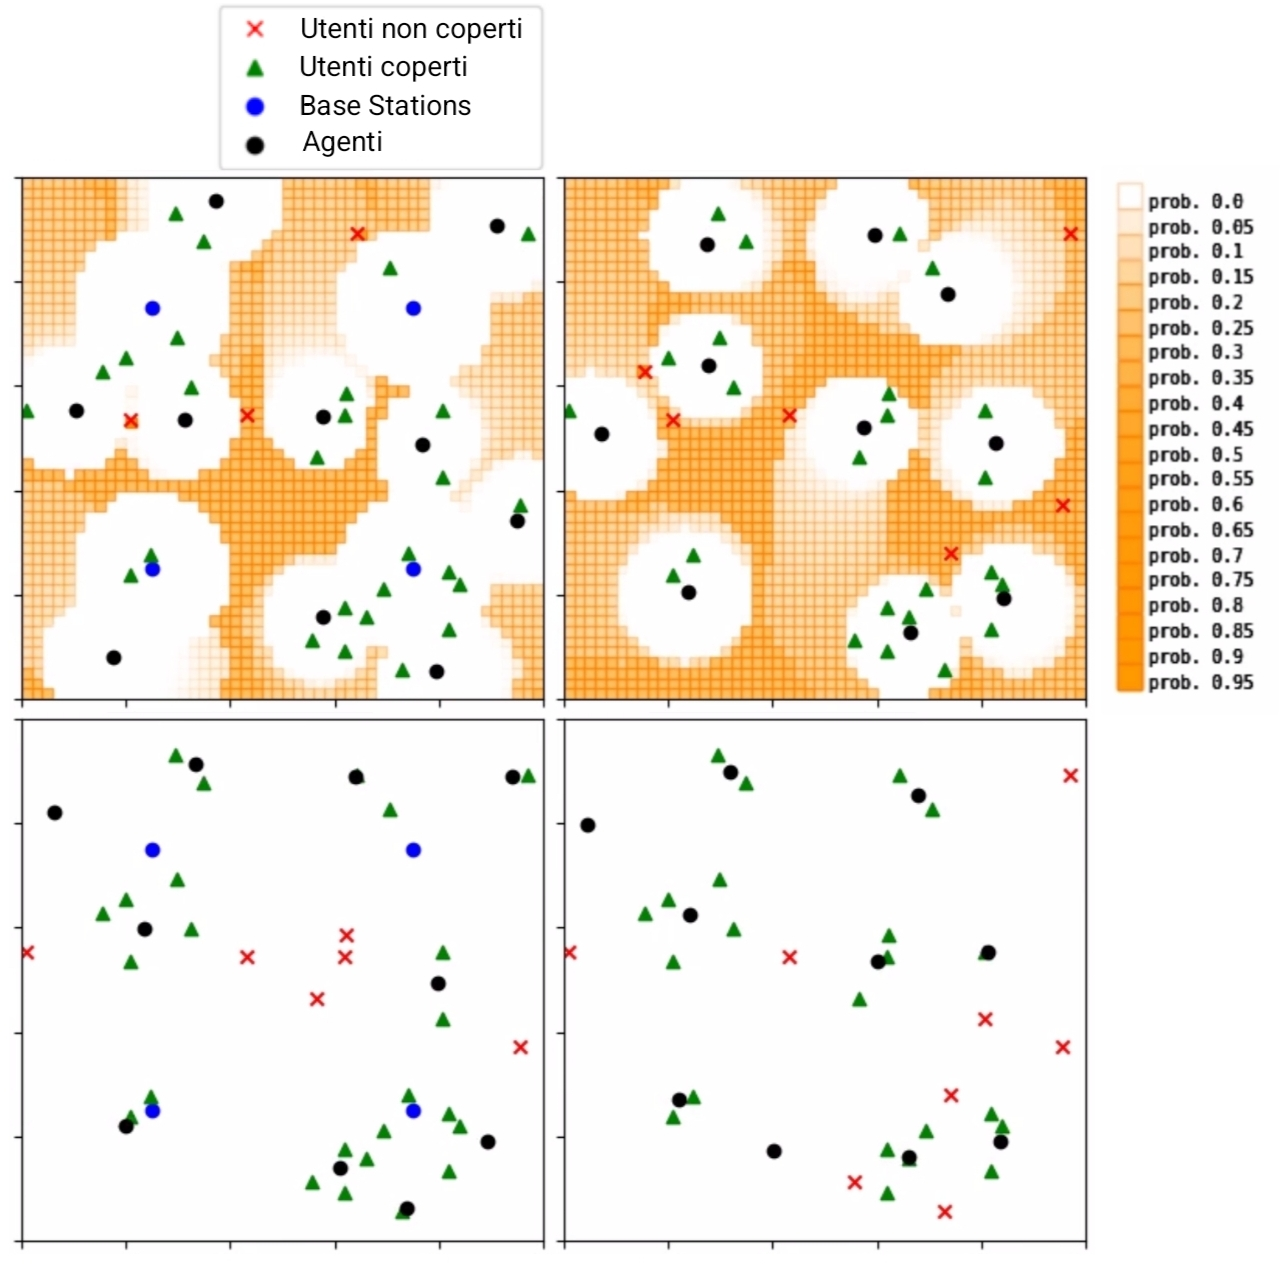
\includegraphics[width=1\linewidth]{img/ch4/experiment1/esempio_simulazioni.jpg}
    \caption[Simulazioni del primo esperimento]{Simulazioni del primo esperimento. In alto a sinistra, lo scenario con esplorazione e con BS; in alto a destra lo scenario con esplorazione ma senza BS; in basso gli scenari senza esplorazione.}
    \label{fig:esempio_simu_exp1}
\end{figure}


\pagebreak
\subsection{Esperimento 2: valutazione del metodo di campionamento migliore}\label{subsec:exp2}
Una volta verificata l'efficacia dell'algoritmo di esplorazione si vuole capire quale, tra le varie tecniche di campionamento, permette di avere dei valori di RCR ed esplorazione migliori.
Data l'uniformità dei risultati precedenti, i seguenti esperimenti sono stati svolti in scenari in cui erano presenti le BS.

\begin{table}[p]
\centering
\begin{tabular}{|c|c|c|c|c|c|}
\hline
Esplorazione & Systematic & Local & Penalty & Ann.forward & Ann.reverse \\
\hline
Massima & 0.86 & 0.87 & 0.86 & 0.87 & 0.86 \\
Minima & 0.79 & 0.79 & 0.79 & 0.81 & 0.81 \\
Media & 0.83 & 0.84 & 0.82 & 0.85 & 0.84 \\
Dev. standard & 0.017 & 0.017 & 0.020 & 0.015 & 0.014 \\
\hline
\end{tabular}
\caption{\label{tab:exp2_expl_statistics}Secondo esperimento, indici dei valori finali di esplorazione.}

\vspace*{0.5 cm}

\begin{tabular}{|c|c|c|c|c|c|}
\hline
Copertura & Systematic & Local & Penalty & Ann.forward & Ann.reverse \\
\hline
Massima & 0.97 & 0.97 & 0.93 & 1 & 0.97 \\
Minima & 0.7 & 0.73 & 0.6 & 0.7 & 0.77 \\
Media & 0.83 & 0.86 & 0.82 & 0.86 & 0.88 \\
Dev. standard & 0.067 & 0.060 & 0.087 & 0.072 & 0.056 \\
\hline
\end{tabular}
\caption{\label{tab:exp2_cov_statistics}Secondo esperimento, indici dei valori finali di copertura.}

\vspace*{0.5 cm}

\begin{tabular}{|c|c|c|c|c|c|}
\hline
 & Systematic & Local & Penalty & Ann.forward & Ann.reverse \\
\hline
tempo medio & 849.3 & 384 & 835.3 & 515 & 495.1 \\
\hline
\end{tabular}
\caption{\label{tab:exp2_time comparison}
Secondo esperimento, tempi medi di esecuzione.}
\end{table}

\begin{figure}[p]
    \centering
    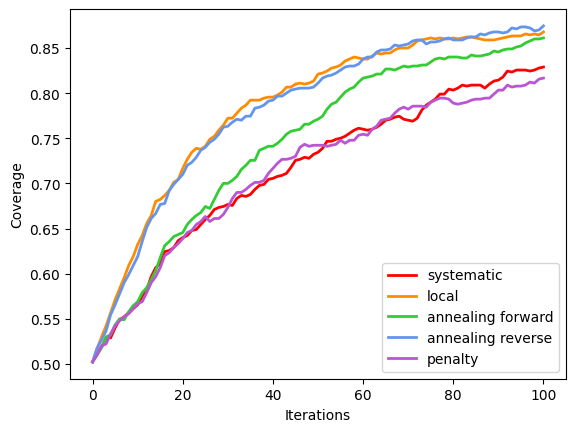
\includegraphics[width=0.8\textwidth]{img/ch4/experiment2/coverages_graphic_comparison.png}
    \caption[Grafici di copertura nel secondo esperimento]{Secondo esperimento, confronto tra i valori medi di copertura utente.}
    \label{fig:confronto_cov_exp2}

\vspace*{0.5cm}

    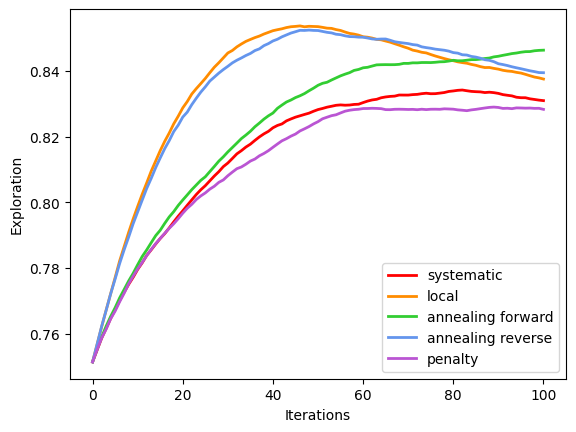
\includegraphics[width=0.8\textwidth]{img/ch4/experiment2/exploration_graphic_comparison.png}
    \caption[Grafici di esplorazione nel secondo esperimento]{Secondo esperimento, confronto dell'andamento medio di esplorazione tra le varie tecniche di campionamento.}
    \label{fig:confronto_expl_exp2}
\end{figure}

Osservando i valori di \textbf{esplorazione} (Figura \ref{fig:confronto_expl_exp2}), si constata che i metodi \textit{local} e \textit{annealing reverse} raggiungo dei livelli molto alti in breve tempo, per poi favorire le posizioni raggiunte dagli agenti.
La tecnica \textit{Annealing forward} invece, a fronte di un transitorio meno rapido, riesce a raggiungere valori finali più alti, come si vede anche in Tabella \ref{tab:exp2_expl_statistics}.
Analizzando i livelli di \textbf{copertura} (Figura \ref{fig:confronto_cov_exp2}), si nota come i metodi \textit{local} e \textit{annealing reverse} risultino i più performanti, sia per i livelli finali raggiunti (Tabella \ref{tab:exp2_cov_statistics}) sia per la velocità di convergenza.
Queste due tecniche sembrano quindi del tutto equivalenti; tuttavia analizzando i tempi di esecuzione in Tabella \ref{tab:exp2_time comparison} si osserva che il tempo della tecnica \textit{local} è circa del 28\% minore rispetto a quello della tecnica \textit{annealing reverse} , portando quindi a favorire la prima per la sua maggiore velocità di esecuzione.

\pagebreak
\subsection{Esperimento 3: variazione della dinamicità dell'ambiente}\label{subsec:exp3}
Fino ad ora gli esperimenti effettuati hanno usato valori di $\mathbb{P_D}$ e $\mathbb{P_B}$ coerenti con un contesto in cui l'informazione relativa al livello di esplorazione in una regione rimane attendibile per un intervallo di tempo relativamente lungo, ovvero coerenti con ambienti aventi bassa dinamicità. 
Con quest'ultimo esperimento dunque si vuole verificare le performance del sistema quando opera in un ambiente maggiormente mutabile nel tempo.
Dati i risultati del precedente esperimento, si è deciso di eseguire queste simulazioni usando solamente la ricerca \textit{local}, confrontando nelle varie prove lo stesso scenario iniziale, ma variando le probabilità di apparizione e disconnessione degli utenti: in un caso si usano i valori definiti in \ref{sec:param_vals}, mentre nell'altro si usano $\mathbb{P_D}=0.01$ e $\mathbb{P_B}=0.07$.

\begin{figure}[p]
    \centering
    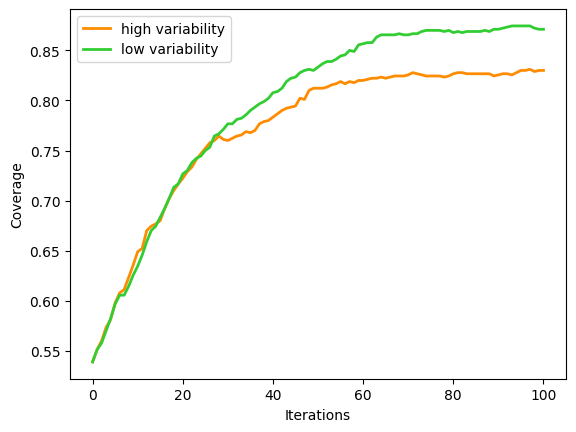
\includegraphics[width=0.8\textwidth]{img/ch4/experiment3/coverages_graphic_comparison.png}
    \caption[Grafici di copertura nel terzo esperimento]{Confronto tra l'andamento medio della copertura negli scenari di simulazione del terzo esperimento.}
    \label{fig:confronto_cov_exp3}

\vspace*{0.5cm}

    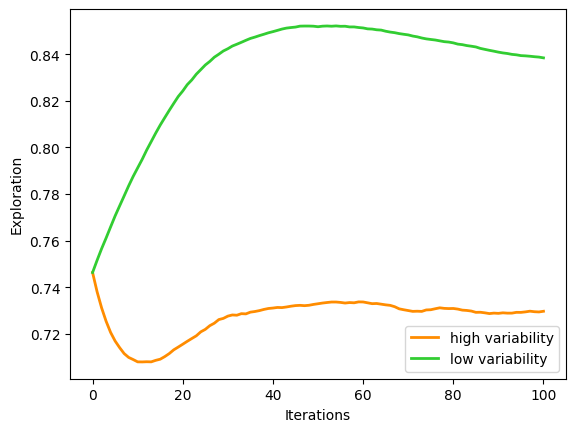
\includegraphics[width=0.8\textwidth]{img/ch4/experiment3/exploration_graphic_comparison.png}
    \caption[Grafici di esplorazione nel terzo esperimento]{Confronto tra l'andamento medio dell'esplorazione negli scenari di simulazione del terzo esperimento.}
    \label{fig:confronto_expl_exp3}
\end{figure}

Analizzando i risultati in Figura \ref{fig:confronto_expl_exp3} notiamo come i livelli di \textbf{esplorazione} diminuiscano drasticamente: questo tuttavia era prevedibile, infatti con questa configurazione la probabilità che appaia un utente in una cella cresce molto rapidamente, e rende impossibile raggiungere alti livelli di esplorazione con la quantità di agenti usati nelle simulazioni.
Per quanto riguarda la \textbf{copertura} (Figura \ref{fig:confronto_cov_exp3}) invece, si riescono a raggiungere dei livelli abbastanza buoni: benché l'algoritmo di esplorazione non impedisca di esplorare ripetutamente alcune zone, è abbastanza flessibile da guidare gli agenti attraverso l'area, disincentivando spostamenti brevi e ripetuti in favore di una traiettoria più pulita.

\begin{figure}
    \centering
    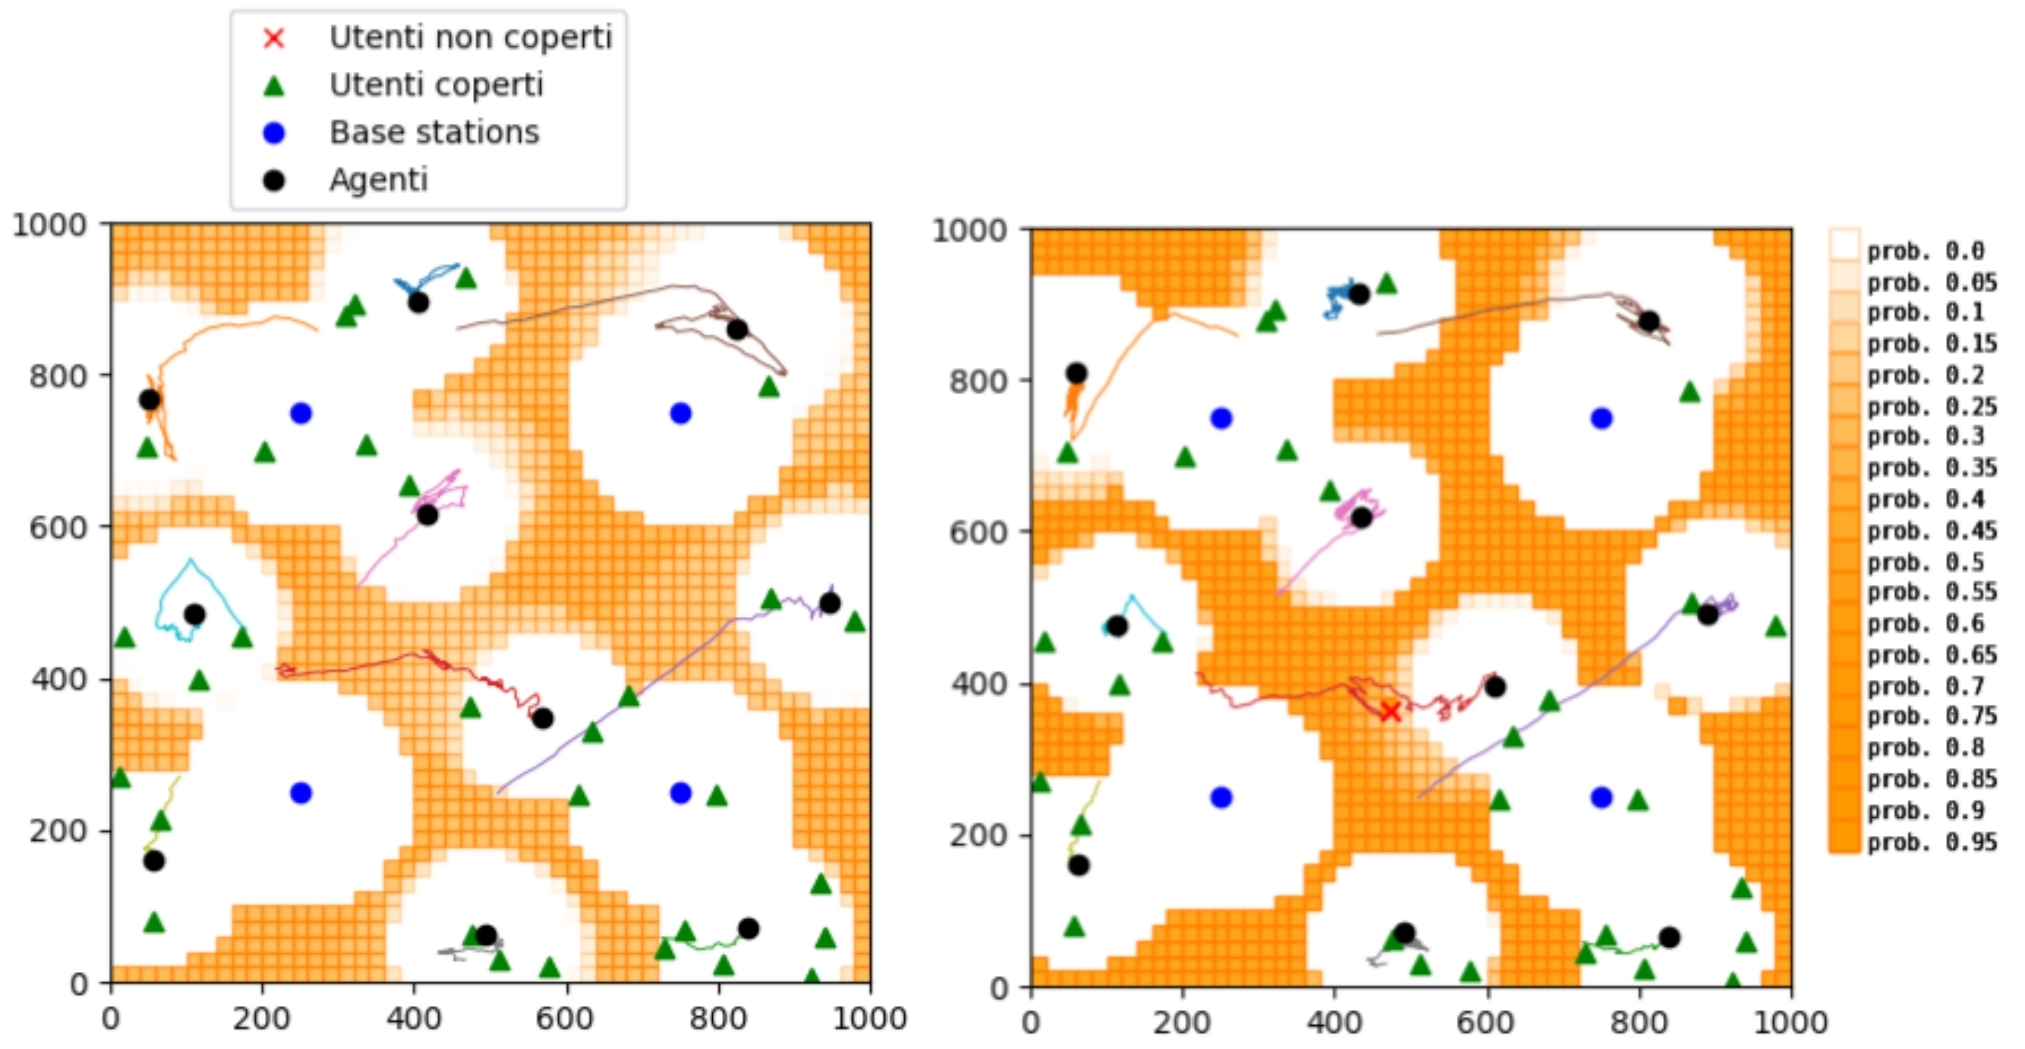
\includegraphics[width=1\linewidth]{img/ch4/experiment3/esempio_exp3_1.jpg}
    \label{fig:esempio_exp3_1}

    \vspace*{0.5cm}
    
    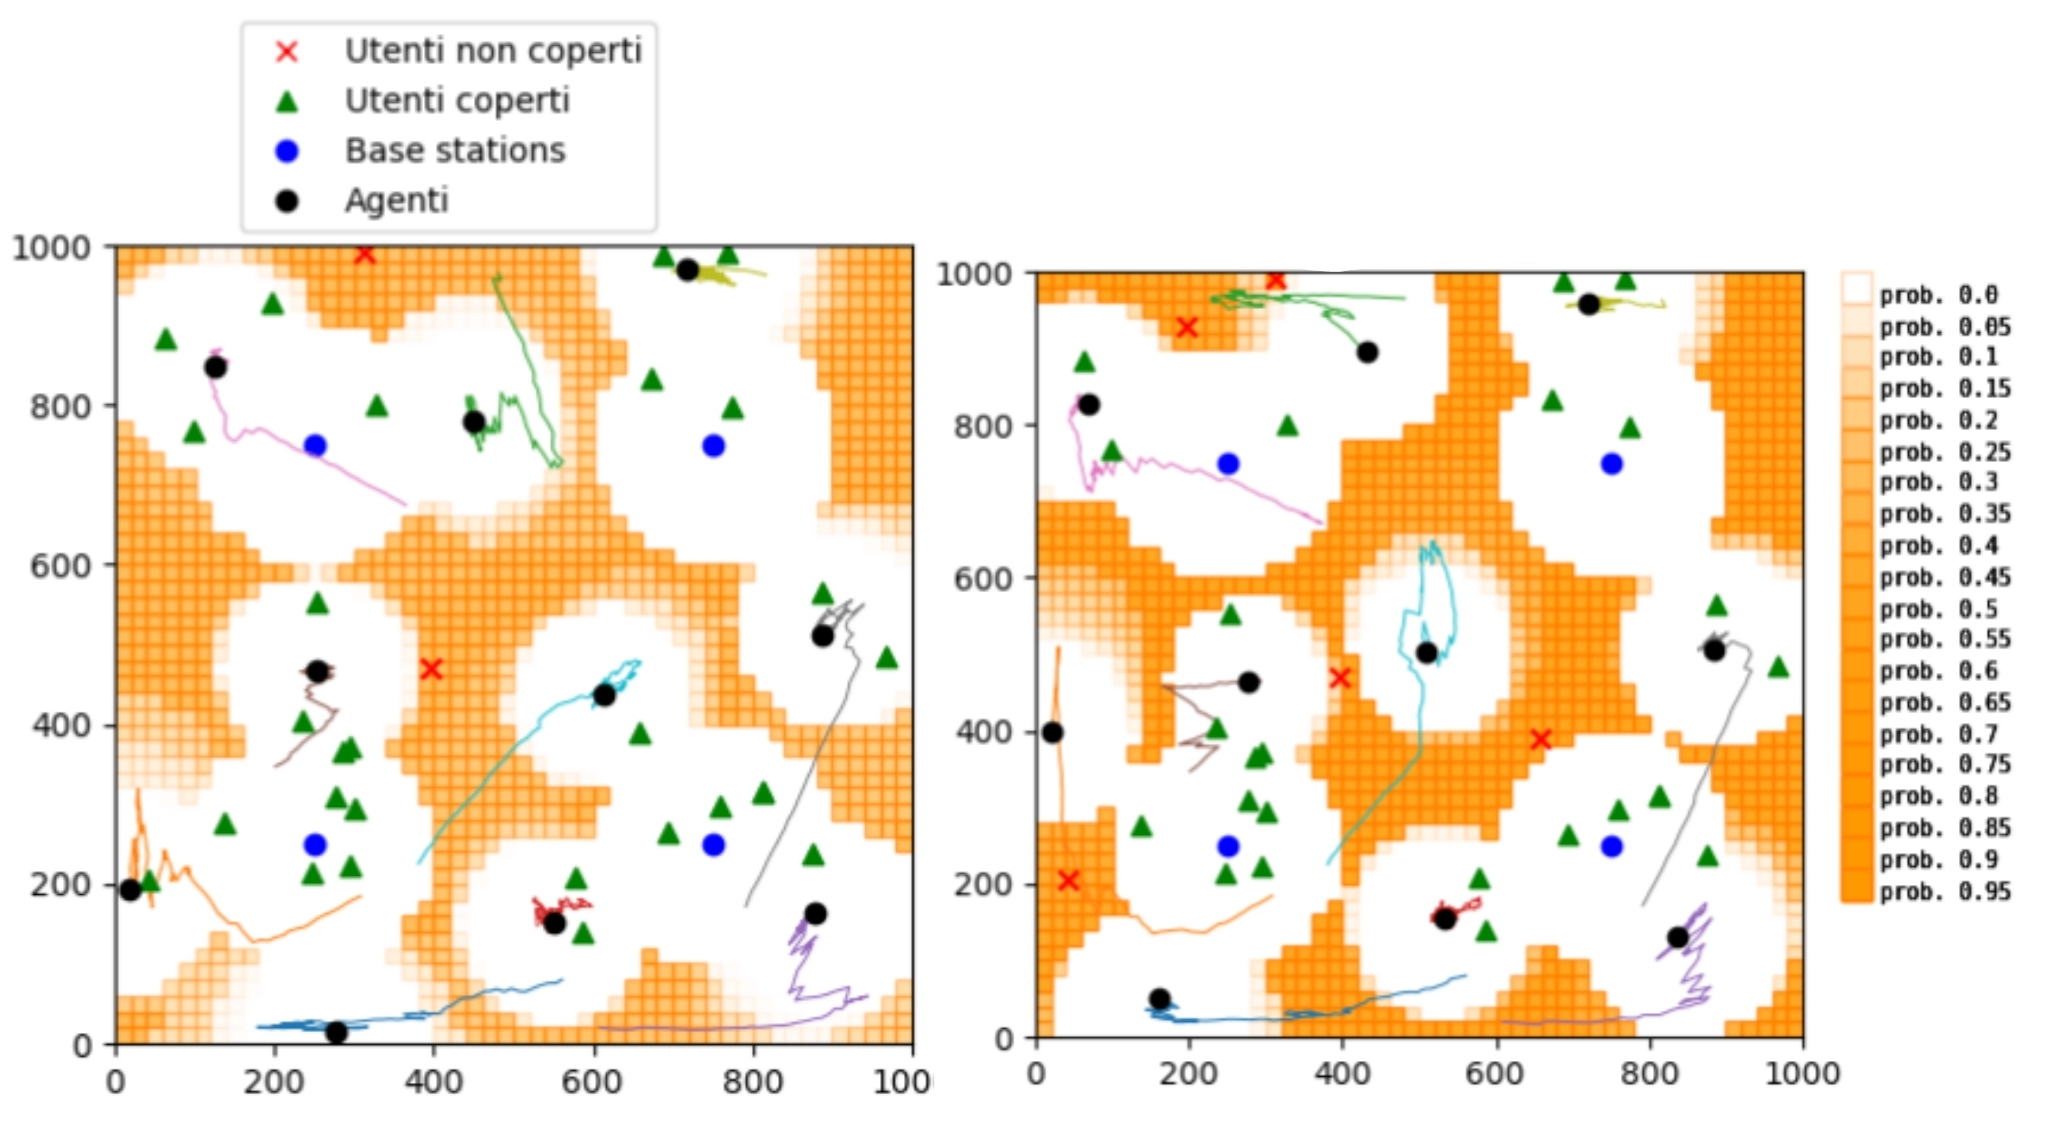
\includegraphics[width=1\linewidth]{img/ch4/experiment3/esempio_exp3_2.jpg}
    \label{fig:esempio_exp3_2}
    \caption[Confronti tra simulazioni con probabilità diverse]{Confronti tra simulazioni con probabilità diverse. Nello scenario di simulazione in alto, nonostante il cambio di parametri le due prove hanno raggiunto livelli di copertura simili. Nello scenario in basso invece la maggiore variabilità dell'ambiente provoca una diminuzione dei risultati raggiunti.}
    
    
\end{figure}
 % 4.2
\chapter{Conclusioni} \label{ch:conclusioni}
Gli esperimenti condotti hanno mostrato come, sotto le ipotesi di non conoscere il numero totale di agenti e che tale numero possa variare, l'algoritmo di esplorazione migliora i risultati ottenuti in termini di utenti coperti rispetto al sistema con il solo algoritmo di copertura.
Inoltre si è verificata l'adattabilità del sistema nel caso in cui venga usato con ambienti molto mutevoli e, nonostante un effettivo calo dei risultati, permette di raggiungere dei risultati accettabili.


Il sistema esposto in questa tesi e le relative analisi coprono solo alcuni casi d'uso, e pertanto le estensioni che è possibile effettuare sono molteplici.
Si potrebbe, per esempio, andare a verificarne il comportamento nel caso in cui gli utenti possano muoversi, senza però che il sistema conosca la frequenza o la lunghezza di tali spostamenti, includendo all'interno dell'algoritmo di controllo un metodo che permetta la stima di tali grandezze mediante un sistema in retroazione.
Oppure si potrebbe rilassare l'ipotesi che l'altitudine sia sufficiente da trascurare eventuali ostacoli orizzontali, e quindi verificare il comportamento del sistema in ambienti più complessi, come quelli urbani, facendo eseguire ai droni spostamenti non più solo bidimensionali, ma anche lungo l'asse verticale.
Un altro aspetto non verificato da questa tesi è quello del consumo energetico, che tuttavia gioca un ruolo fondamentale nei sistemi reali e che potrebbe essere incluso nel modello bilanciando il guadagno che si ottiene a seguito di uno spostamento con il suo consumo energetico.
Infine, è possibile sperimentare nuovi metodi per l'esplorazione, usando anche tecniche di machine learning, fra cui il reinforcement learning.

\addcontentsline{toc}{chapter}{Bibliografia}
%\bibliography{biblio}
\printbibliography

\addcontentsline{toc}{chapter}{Elenco delle figure}
\listoffigures   % inserisce indice figure
\addcontentsline{toc}{chapter}{Elenco delle tabelle}
\listoftables    % inserisce indice tabelle
\addcontentsline{toc}{chapter}{Elenco degli snippet}
\lstlistoflistings

\chapter*{Ringraziamenti}
\addcontentsline{toc}{chapter}{Ringraziamenti}

In primis un ringraziamento va al mio relatore e al mio corelatore per l'opportunità che mi hanno dato di lavorare su un progetto estremamente affascinante.
Ringrazio la mia famiglia, e soprattutto ringrazio i miei genitori, per avermi permesso di intraprendere questa strada ed avermi supportato durante il tragitto.
Ringrazio i miei amici, quelli conosciuti all'università, quelli conosciuti agli scout e quelli conosciuti altrove, e in particolare voglio ringraziare coloro che sono sempre rimasti al mio fianco: Cosimo, Gianmarco e Vincenzo, un grazie in più è tutto per voi. 
Infine voglio ringraziare Agnese, più di tutti mi sei stata accanto in questo periodo, mi hai sopportato e aiutato,  mi hai sempre ascoltato anche quando ero troppo arrogante da credere di non averne bisogno. Grazie.

\end{document}
